\documentclass[preprint,authoryear,10pt]{elsarticle}

% -------------------- 1. Formatting & Encoding --------------------
\usepackage[utf8]{inputenc}
\usepackage[T1]{fontenc}
\usepackage[margin=1.2in]{geometry}
\usepackage{microtype}      % Improves typography
\usepackage{xcolor}         % Color management
\usepackage{enumitem}       % Custom lists
\usepackage{float}          % Better float control

% -------------------- 2. Mathematics & Units --------------------
\usepackage{amsmath,amssymb,bm}
\usepackage{siunitx}
\sisetup{
    detect-all,
    group-minimum-digits=4,
    group-separator={\,},
    inter-unit-product=\ensuremath{{\cdot}}
}
\DeclareSIUnit{\kmh}{km/h}

% -------------------- 3. Tables & Graphics --------------------
\usepackage{graphicx}
\usepackage{booktabs}       % Professional table rules
\usepackage{threeparttable} % Tables with footnotes
\usepackage{multirow}
\usepackage{makecell}
\usepackage{tabularx}
\usepackage{longtable}
\usepackage{array}
\usepackage{caption}
\usepackage{subcaption}
\usepackage{comment}

% Custom Column Types
\newcolumntype{F}[1]{>{\raggedright\arraybackslash\hspace{0pt}}p{#1}}
\newcolumntype{T}[1]{>{\centering\arraybackslash\hspace{0pt}}p{#1}}

% -------------------- 4. Hyperlinks (Load Last) --------------------
\usepackage[colorlinks=true, urlcolor=blue, linkcolor=red, citecolor=green]{hyperref}

% -------------------- Journal Metadata --------------------
\journal{Transportation Research Part C} 

\begin{document}

\begin{frontmatter}

% -------------------- Title --------------------
\title{A Multi-Objective Framework for Cycling Infrastructure Decisions}

% -------------------- Authors & Affiliations --------------------
    
    % Author 1: Narges Ahmadi (Corresponding)
    \author[mcgill]{Narges Ahmadi\corref{cor1}}
    \ead{narges.ahmadi@mail.mcgill.ca}
    
    % Author 2: Jônatas Augusto Manzolli
    \author[mcgill,inescc]{Jônatas Augusto Manzolli}
    \ead{jonatas.manzolli@mcgill.ca}
    
    % Author 3: Jiangbo Yu
    \author[mcgill]{Jiangbo Yu}
    \ead{jiangbo.yu@mcgill.ca}
    
    % Author 4: Luis Miranda-Moreno
    \author[mcgill]{Luis Miranda-Moreno}
    \ead{luis.miranda-moreno@mcgill.ca}
    
    % Correspondence Footnote
    \cortext[cor1]{Corresponding author}
    
    % Affiliation Address
    \address[mcgill]{Department of Civil Engineering, McGill University, Montreal, QC, Canada}
    \address[inescc]{INESC Coimbra, University of Coimbra, Coimbra, Portugal}

% -------------------- Abstract --------------------
\begin{abstract}

Station-based bike-sharing and cycling infrastructure are often planned separately, creating mismatches between station demand and comfortable network access. This study develops a tri-objective optimization framework that jointly selects bikeway upgrades and station deployment to maximize demand coverage, minimize traffic stress, and limit cost. Applied to Montreal's 30 highest-activity downtown stations, the results show strong but nonlinear trade-offs. A balanced solution serves 4.613 million trips with 93 stations and 72 links, capturing most of the attainable demand while avoiding the extreme stress and cost of the demand-maximizing design. The normalized sensitivity analysis shows that requiring more stations increases demand per station only slightly, from 48,603 to 49,608, while worsening stress per link from 1.78 to 1.98. Requiring more links leaves demand per station nearly unchanged, from 49,008 to 49,597, but raises cost per infrastructure element from 4,562.5 to 6,273.2. The results support targeted investment in high-demand, low-stress corridors.

\end{abstract}

 % -------------------- Keywords --------------------
\begin{keyword}
    Bike-sharing systems \sep 
    Multi-objective optimization \sep 
    Bicycle infrastructure planning \sep 
    Level of Traffic Stress \sep 
    Origin–destination demand
\end{keyword}

\end{frontmatter}

% -------------------- Main Content --------------------
% -------------------- Intro --------------------

\section{Introduction}\label{intro}

Cycling is a core component of sustainable urban mobility. Reducing reliance on motorized travel supports lower emissions and improved air quality, while also delivering public health benefits through regular physical activity \citep{CHEN2022103475, BRAND2021102764}. Station-based bike-sharing systems further strengthen this promise by expanding access to bicycles, enabling short urban trips with low energy use and zero tailpipe emissions \citep{Pucher02112017, MCQUEEN2020102482, JACOBSON200914}. Despite these benefits, bikeway infrastructure and station-based bike-sharing systems are commonly planned as separate investments, often guided by different objectives, data sources, and implementation timelines. This separation can produce networks in which stations are placed in high-demand areas that remain weakly connected to comfortable routes, or in which new bike lanes fail to connect to stations that could sustain usage. Existing planning approaches therefore struggle to coordinate three interdependent dimensions that shape system effectiveness: where people want to travel (demand), whether they feel safe and comfortable doing so (traffic stress), and what can realistically be built within fiscal constraints (budget) \citep{wiedemann2025Bikenetworkplanning, paulsen2023Societallyoptimalexpansion, nateraorozco2020Datadrivenstrategiesoptimal}. Furthermore, because cyclists strongly prefer protected, continuous, and well-connected routes with low exposure to traffic stress \citep{buehler2016BikewayNetworksReview, ta2021impactgreenspace, GRAYSTONE2022103237}, misalignment between stations and low-stress connectivity can erode user confidence and suppress ridership, thereby reducing the returns to otherwise well-intentioned investments.

Motivated by these gaps, this study develops a multi-objective optimization framework for integrated planning of bicycle infrastructure and station-based bike-sharing systems. The framework jointly maximizes Origin-Destination (OD) demand coverage, minimizes cyclist exposure to Level of Traffic Stress (LTS), and accounts for procurement costs associated with link upgrades and station deployment. By combining these elements within a single decision model, the approach enables planners to prioritize investments transparently and to explore how alternative policy preferences shift the balance between coverage, comfort, and cost. To the best of the authors' knowledge, these dimensions have not been evaluated jointly within a unified optimization framework for coordinated bikeway and station planning. The main contributions of this study are as follows:

\begin{itemize}
\item Proposing a multi-objective optimization model that jointly designs bikeway upgrades and bike-share station deployment, solved using an evolutionary algorithm.
\item Integrating OD demand estimation and LTS evaluation directly into the optimization process to improve planning relevance and interpretability.
\item Demonstrating practical applicability through a Montreal case study, revealing trade-offs between coverage, comfort, and cost.
\item Assessing robustness through sensitivity analyses across budgetary and infrastructure scenarios.
\end{itemize}

The paper is organized as follows. Section~\ref{review} reviews literature on cycling accessibility and infrastructure planning. Section~\ref{method} presents the methodological approach, including data acquisition and model formulation. Section~\ref{casestudy} describes the Montreal case study. Section~\ref{results} discusses the results, including Pareto-optimal outcomes and sensitivity analyses. Section~\ref{policy} presents policy-making directions stemming from the results of the optimization experiments. Section~\ref{conclusion} concludes with key takeaways, limitations, and directions for future research.

% -------------------- Review --------------------

\section{Literature Review}\label{review}

This section positions the proposed framework within three interconnected research streams. First, we review how bicycle network design and connectivity influence ridership and safety, and how comfort is operationalized through stress-based indicators. Second, we summarize approaches to bike-sharing system planning, with emphasis on station placement and demand representation. Third, we synthesize optimization-based models that formalize these planning problems, highlighting methodological trends in multi-objective design, uncertainty, and equity. The section concludes by identifying the specific integration gap addressed by this paper.

\subsection{Design and Connectivity of Bicycle Networks}

Bicycle network design influences cycling uptake primarily through perceived safety, continuity, and route directness. A consistent finding in the literature is that dedicated facilities such as protected bike lanes and cycle tracks are associated with higher cycling mode share and increased trip frequency \citep{mitra2017Modesubstitutioneffect, dill2003BicycleCommutingFacilities, buehler2012Cyclingwork90}. However, these benefits are not uniform across users. Cyclists differ in experience, risk tolerance, and comfort thresholds, motivating typologies that capture heterogeneous infrastructure preferences \citep{dill2013FourTypesCyclists, damant-sirois2014WhatsYourType}. This heterogeneity implies that networks designed around confident riders may not attract stress-sensitive groups, limiting broader mode shift. Connectivity is a complementary determinant of cycling adoption. Empirical evidence shows that cyclists prefer direct, continuous routes with minimal detours, since discontinuities reduce convenience and can increase exposure to stressful traffic interactions \citep{schoner2014missinglinkbicycle, fitch2022Whatmakesbicyclists, dill2009BicyclingTransportationHealth, reggiani2022Understandingbikeabilitymethodology}. As a result, planning efforts increasingly emphasize coherent low-stress networks that support end-to-end trips rather than isolated segments \citep{rayfield2011Connectivityconservationframework}.

To evaluate network quality, several indicators have been proposed. Early methods include the Bicycle Compatibility Index (BCI) \citep{harkey1998DevelopmentBicycleCompatibility} and Bicycle Level of Service (BLOS) approaches that score segments using traffic conditions and geometric attributes \citep{jensen2007PedestrianBicyclistLevel, petritsch2007BicycleLevelService}. Extensions such as the Munich Bikeability Index integrate additional criteria and GIS-based workflows \citep{schmid-querg2021MunichBikeabilityIndex}. While useful for diagnosis, many score-based approaches provide limited interpretability for specific user groups and are less suited to identifying ``usable'' low-stress connectivity.

To address these limitations, \citet{mekuria_low-stress_2012} introduced the LTS framework, which classifies segments based on the degree of traffic interaction that different users are likely to tolerate, using a weakest-link logic. LTS has become a practical standard for mapping low-stress connectivity and identifying network gaps. In this study, LTS is adopted as the primary comfort metric because it provides an interpretable representation of network usability that can be embedded into optimization-based planning.

\subsection{Bike-Sharing System Planning}

Bike-sharing planning involves strategic decisions such as station location, station density, and capacity design, often coupled with operational challenges such as rebalancing and demand variability. A key methodological trend is the use of data-driven demand estimation and optimization to improve service performance and equity. For example, recent work has proposed robust and stochastic formulations that explicitly account for demand uncertainty and service fairness \citep{chen2023target, nikiforiadis2021determining, jin2020Robustbikesharingstations}. Complementary approaches integrate predictive models, including machine learning, to estimate station-level demand and support station siting decisions \citep{7373406}. Multi-objective formulations are also common in this domain, particularly when balancing service quality against operational costs such as redistribution \citep{8932534, soriguera2020continuous}.

While this literature provides powerful tools for station placement and operations, bike-sharing is often modeled as a system operating atop an assumed underlying bikeway environment. As a result, station plans may not explicitly account for whether users can access stations via low-stress routes, which can be critical for sustained usage and user confidence.

\subsection{Optimization Models for Bicycle Infrastructure and Bike Systems}

Optimization models have been widely used to support bicycle system planning, spanning strategic network design, station placement, fleet sizing, and operational rebalancing \citep{laporte2018Sharedmobilitysystems, shui2020reviewbicyclesharingservice}. Foundational work formulated Mixed-Integer Linear Programming (MILP) models to decide station locations and fleet size for real-world systems \citep{lin2011Strategicdesignpublic, martinez2012OptimisationAlgorithmEstablish, frade2015Bikesharingstationsmaximal, garcia-palomaresOptimizingLocationStations2012}. More recent studies extend these formulations to incorporate network structure and perceived comfort, using graph-based connectivity measures to target upgrades that improve usability \citep{10920161}.

Methodologically, three themes are particularly relevant to this paper. First, robust and stochastic formulations address uncertainty in demand and system performance, often through multi-scenario planning \citep{jin2020Robustbikesharingstations, yan2017Rentalbikelocation}. Second, multi-objective optimization is increasingly used to make trade-offs explicit, particularly between service coverage and cost \citep{vishkaei2021Biobjectiveoptimizationcustomers, fan2024Takingmultimodalapproach}. Third, equity-aware models introduce constraints or objective terms that regulate disparities in access and service levels across neighborhoods or population groups \citep{caggiani2020approachmodelingbikesharing, duran-rodas2021DemandEquityDARE, behbahani2019conceptualframeworkformulate}. These advances suggest a maturing field, but also reveal that different components of the cycling ecosystem are often optimized in isolation.

\subsection{Research Gap}

Despite growing attention to active transportation, the integrated planning of bikeway infrastructure and bike-sharing systems remains limited. Most bike-sharing models focus on station placement, fleet sizing, or rebalancing while treating the bikeway environment as fixed. Conversely, bicycle infrastructure planning typically prioritizes connectivity and comfort but does not jointly determine station locations or account for observed OD demand mediated by station access. In addition, while LTS is widely used for diagnostic mapping of low-stress networks, it is less commonly embedded as an explicit objective component within optimization models that also incorporate demand coverage and procurement costs.

These gaps are particularly consequential in dense urban settings where trade-offs between coverage, comfort, and budget are unavoidable. This study addresses the above limitations by proposing and validating a multi-objective optimization framework that jointly considers OD demand, LTS-based comfort, and cost constraints, and co-optimizes bikeway upgrades and bike-share station deployment.


% -------------------- Methodology --------------------


\section{Methodology}\label{method}

In this section, we present the methodological framework used in this paper, which is divided into four main steps: (i) data processing, (ii) optimization model design, (iii) case study evaluation, and (iv) sensitivity analysis. Figure \ref{framework} details the main actions applied in our framework.

\begin{figure}[htbp]
  \centering
  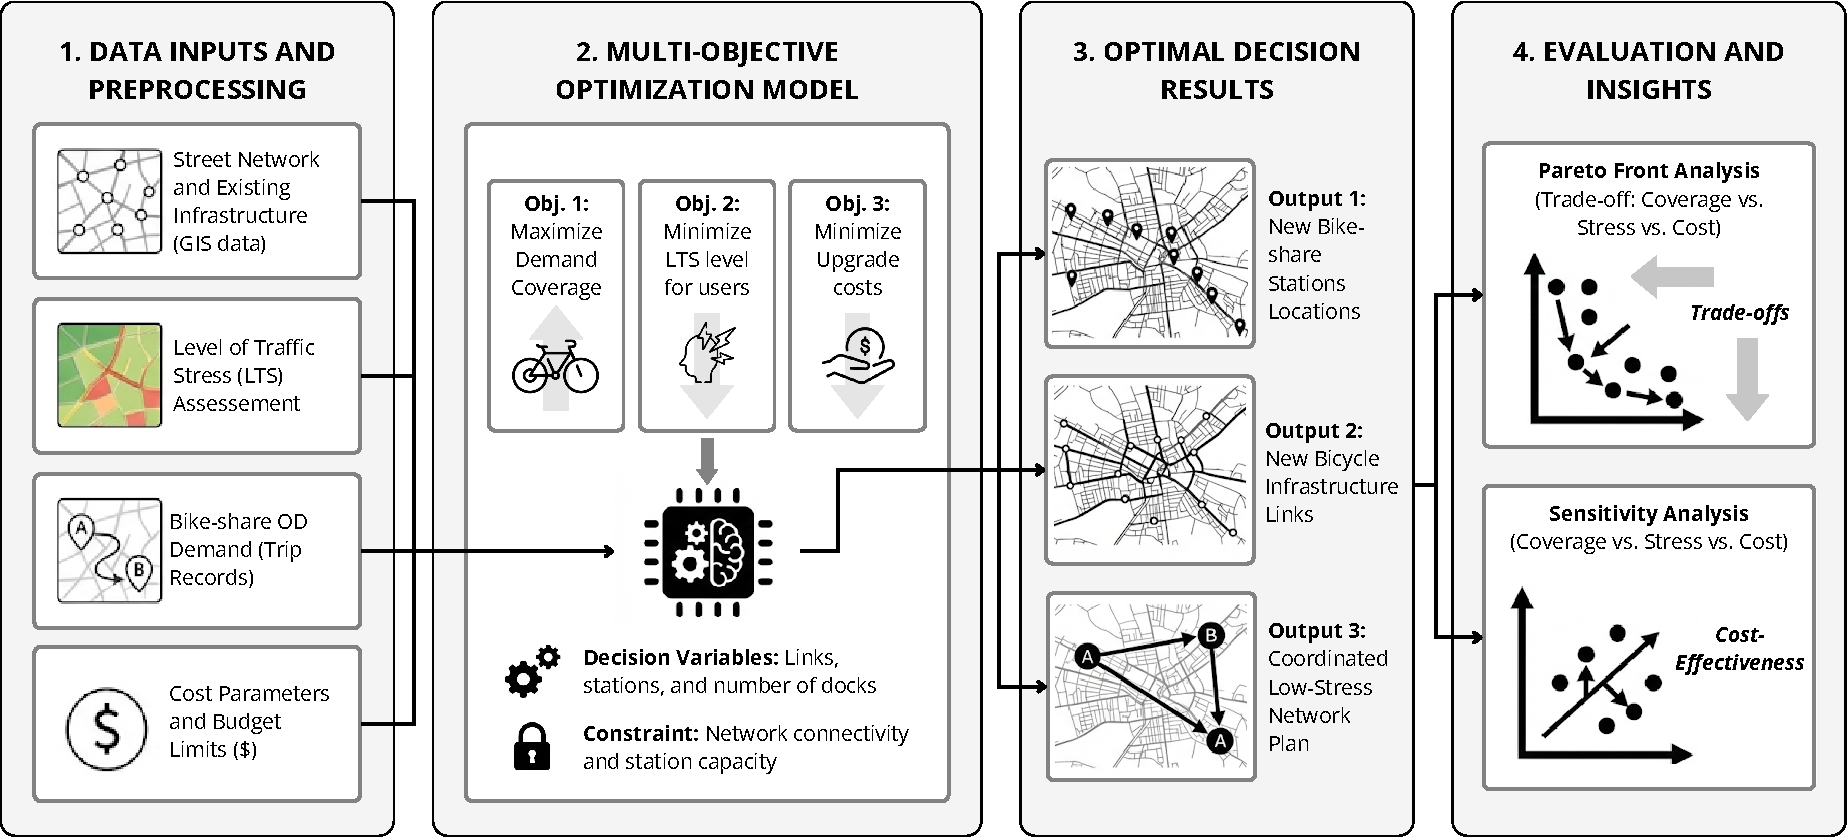
\includegraphics[width=1\textwidth]{Figures/framework.pdf}
  \caption{Framework applied in this paper.}\label{framework}
\end{figure}

The proposed methodology provides a systematic and integrated workflow for bicycle infrastructure planning. \textbf{(i) Data inputs and preprocessing:} We compile and harmonize the main inputs required by the model, including LTS values for candidate links derived in a GIS environment and OD-based cycling demand estimates. \textbf{(ii) Multi-objective optimization model:} We then formulate a multi-objective MILP that co-optimizes bikeway upgrades and station-based supply by maximizing demand coverage while minimizing network-wide traffic stress and procurement costs, subject to operational and budget constraints. A weighted-sum scalarization is employed to generate Pareto-efficient solutions and to make policy trade-offs transparent. \textbf{(iii) Optimal decision results:} Next, the model is applied to the Montreal case study, and solutions are translated into implementable designs that specify upgraded links, activated station locations, and dock allocations. \textbf{(iv) Evaluation and insights:} Finally, we conduct sensitivity analyses to quantify how changes in budget levels and key infrastructure parameters influence demand coverage, comfort outcomes, and investment decisions.

Together, these steps provide actionable guidance by identifying cost-effective interventions that improve both network usability and service coverage. The remainder of this section details each component of the methodological approach.

\subsection{Cycling Data Inputs and Preprocessing}

The data acquisition process involved integrating multiple sources to support both the demand modeling and infrastructure assessment components of this study. We collected detailed spatial and trip-level datasets to characterize the current cycling network and inform the development of the optimization model. These datasets were cleaned and processed to ensure compatibility across the analysis. Two primary inputs, namely cycling OD demand and LTS, formed the basis for constructing a realistic infrastructure planning framework.

%\subsubsection{Cycling Demand Acquisition}

Cycling demand is a key input to the proposed optimization framework because both station deployment and bikeway upgrades should reflect trip origins and destinations. To quantify this demand, we used the publicly available trip-level records from Montreal’s BIXI open data\footnote{More at: \url{https://bixi.com/en/open-data/}}, which report daily origin and destination stations, timestamps, and other relevant trip attributes. Figure \ref{fig:bixi_examples} illustrates a typical BIXI station and the spatial footprint of the current station network.

\begin{figure}[htbp]
    \centering
    \begin{subfigure}[b]{0.48\textwidth}
        \centering
        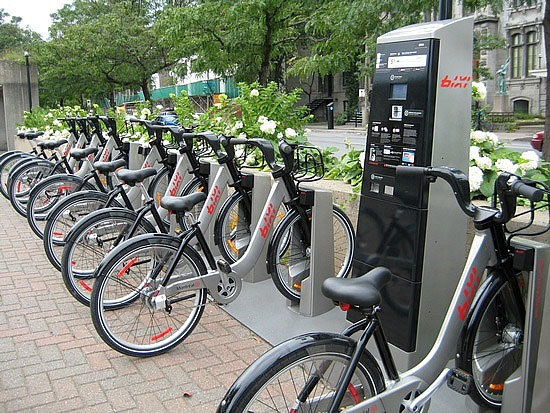
\includegraphics[width=\textwidth]{Figures/Bikesharing-BIXI-in-Montreal-see-online-version-for-colours.png}
        \caption{BIXI station with parked bicycles.}
        \label{fig:bixi_station}
    \end{subfigure}
    \hfill
    \begin{subfigure}[b]{0.425\textwidth}
        \centering
        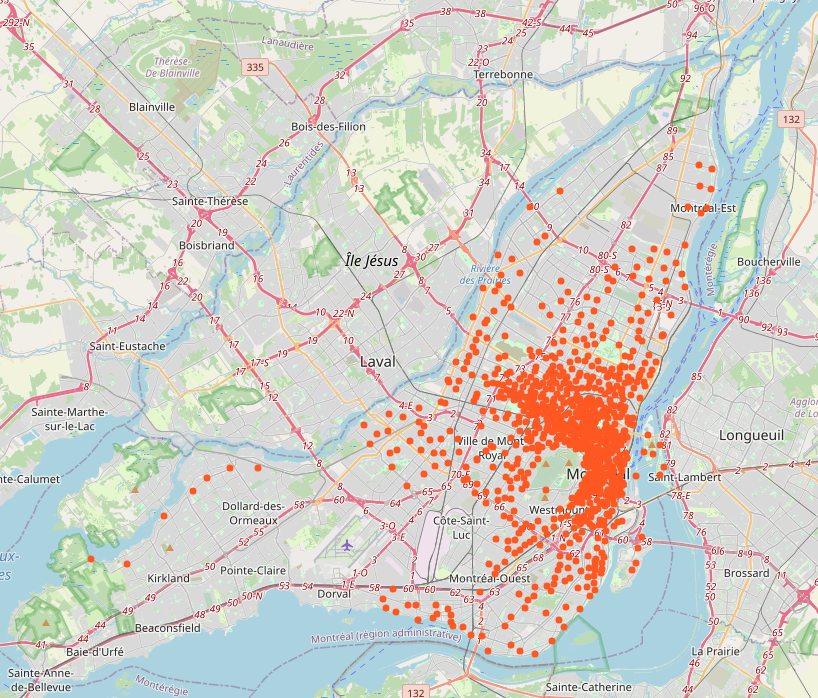
\includegraphics[width=\textwidth]{Figures/BIXI_Stations.png}
        \caption{Map of BIXI stations.}
        \label{fig:bixi_map}
    \end{subfigure}
    \caption{Illustrative examples of Montreal’s BIXI bike-sharing system.}
    \label{fig:bixi_examples}
\end{figure}

We extracted and processed OD trip records spanning multiple months of system operation and aggregated inbound and outbound activity at each station to construct a spatial demand surface. To link observed demand to candidate station locations in the optimization model, we defined service catchments around each station using circular buffers. A radius of 400~m was adopted, consistent with commonly used access distances in the bike-sharing literature \citep{el2017effects}. Demand within each catchment was computed by summing the numbers of trip origins and destinations associated with stations within the buffer, yielding a zonal estimate of cycling activity directly compatible with the candidate infrastructure graph.

Prior to aggregation, the dataset was cleaned to remove incomplete or implausible records, including trips with missing timestamps, invalid station identifiers, or zero duration. Station metadata was inferred by extracting unique station entries from the trip data. The resulting station-level demand estimates were then used to parameterize the optimization problem, ensuring that selected stations and upgraded links prioritize locations with demonstrated usage intensity and reflect observed travel behavior in the Montreal bike-sharing system.


\subsection{Level of Traffic Stress}\label{subsec:lts}

LTS classifies road segments and intersections into discrete stress levels based on operational and geometric characteristics, including motor-vehicle speed, traffic volume, number of travel lanes, and the presence and type of cycling infrastructure. This rider-centered approach is particularly relevant for cities aiming to increase mass cycling by attracting the large population segment characterized as \textit{interested but concerned} (Geller, 2006), rather than designing exclusively for confident riders. LTS thus provides an interpretable basis for identifying corridors likely to discourage stress-sensitive users and for prioritizing infrastructure upgrades that improve network usability and inclusivity.

\subsubsection{LTS Framework and Classification}\label{subsubsec:lts_definition}

The LTS framework classifies each road segment into one of four stress levels reflecting the tolerance of different cyclist groups. LTS~1 represents conditions suitable for all ages and abilities, while LTS~4 represents conditions appropriate only for very confident riders (see Figure \ref{fig:lts_levels}). This classification is grounded in empirical research on cyclist comfort and behavioral response to traffic stress (Mekuria et al., 2012; Furth et al., 2016) and has become standard in cycling network planning practice.

\begin{figure}[htb]
    \centering
    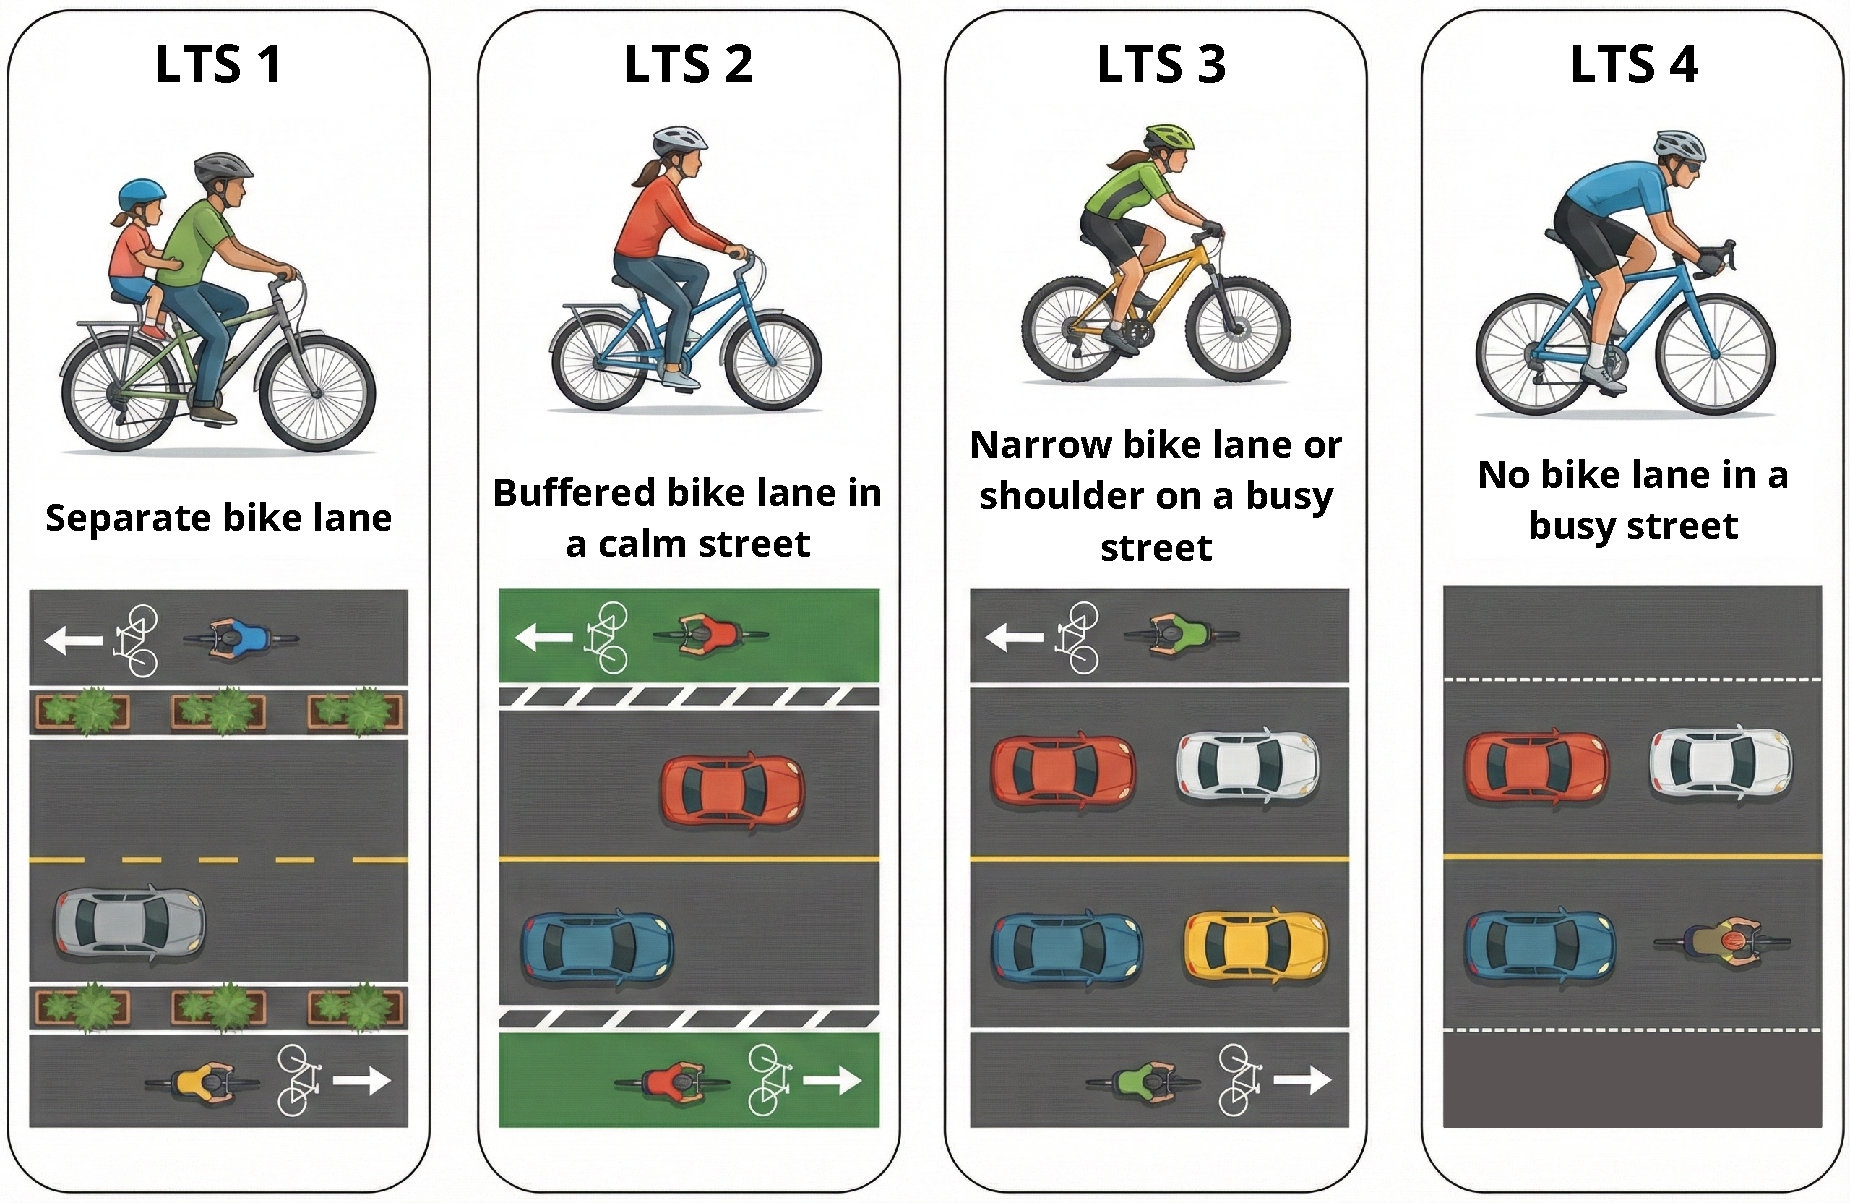
\includegraphics[width=1.0\textwidth]{Figures/lts.pdf}
    \caption{Illustration of the four LTS levels, from LTS~1 (all ages and abilities) to LTS~4 (very confident riders only).}
    \label{fig:lts_levels}
\end{figure}

The LTS classification is determined by evaluating four primary criteria: motor-vehicle speed, traffic volume, number of travel lanes, and bicycle infrastructure type and quality. Table~\ref{tab:lts_criteria} summarizes the evaluation thresholds for each LTS level. The framework prioritizes direct measures of speed and volume over functional-class proxies, as functional classes may misrepresent actual conditions---for example, a local street may carry several thousand vehicles per day in urban contexts, generating substantial stress despite its nominal classification. Recent refinements to the LTS framework (e.g., LTS~v2.0 and later versions) have improved representation of low-speed, high-volume streets and mixed-traffic conditions, addressing limitations that arise when applying the framework in large urban areas.

\begin{table}[htbp]
    \centering
    \small
    \caption{LTS evaluation criteria.}
    \label{tab:lts_criteria}
    \begin{tabularx}{\textwidth}{@{} l l l l l X @{}}
        \hline
        \textbf{LTS} & \textbf{Target Users} & \textbf{Speed} & \textbf{Volume} & \textbf{Lanes} & \textbf{Infrastructure} \\
        \hline
        1 & All ages and abilities & $\leq 40$ km/h & Low & $\leq 1$/direction & Separated facilities or quiet streets \\
        2 & Most adults, not children & $\leq 50$ km/h & Moderate & $\leq 2$/direction & Protected or painted bike lanes \\
        3 & Experienced cyclists & $\leq 60$ km/h & High & Multiple & Shared lanes, minimal facilities \\
        4 & Very confident cyclists & $> 60$ km/h & Very high & Multiple & No infrastructure, arterials \\
        \hline
    \end{tabularx}
\end{table}

\subsubsection{LTS Measurement and Mapping for Montreal}\label{subsubsec:lts_montreal}
 
Implementing network-wide LTS mapping requires overcoming a fundamental data challenge: obtaining reliable, spatially complete measures of traffic speed and volume across the entire study area. Functional-class proxies prove insufficient in urban contexts, where streets nominally classified as local may carry several thousand vehicles per day. To produce an LTS classification that reflects actual traffic conditions, we implemented a three-step, data-driven methodology combining empirical data sources, targeted validation, and automated classification. Figure \ref{fig:lts_framework} summarizes the framework.

\begin{figure}[htbp]
    \centering
    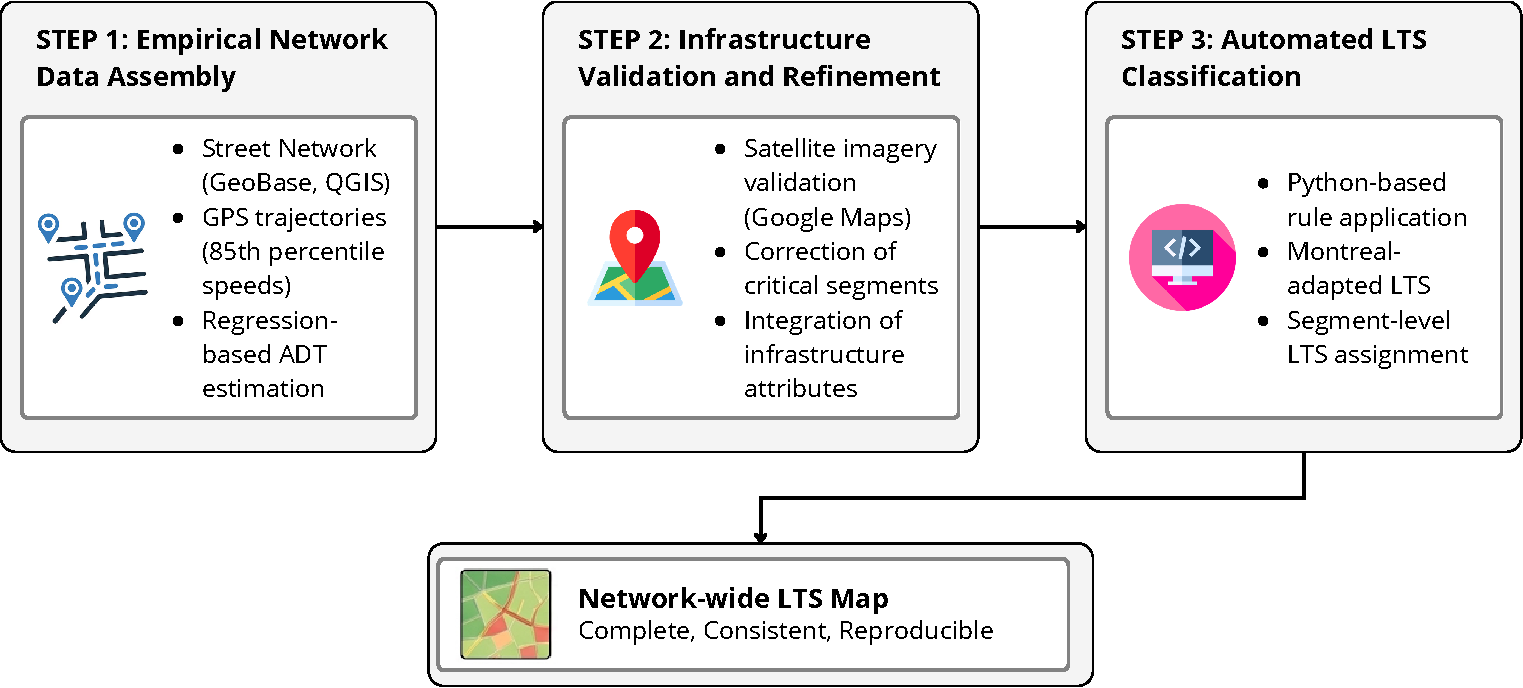
\includegraphics[width=1\linewidth]{Figures/lts_framework.pdf}
    \caption{LTS calculation framework.}
    \label{fig:lts_framework}
\end{figure}

This three-step approach (empirical data assembly, strategic validation, and transparent, automated classification) produced a network-wide LTS mapping that is comprehensive, defensible, and reproducible. In the following, we detail each step:
\\
\\
\textbf{Step 1 -- Network Assembly and Empirical Speed and Volume Data:} We began by constructing a street-segment network for the Island of Montreal in QGIS, using the City of Montreal's GeoBase as the foundation. Rather than inferring speed and volume from functional class, these variables were derived from empirical data. Where direct traffic counts and speed measurements were unavailable, full spatial coverage was achieved using large-scale GPS trajectory data (myDrive, Intact Insurance). Off-peak 85th-percentile vehicle speeds were computed for each segment to represent typical conditions without transient congestion. Average Daily Traffic (ADT) was estimated using regression models calibrated to observed traffic counts and adjusted for functional class, number of lanes, and one-way operation. This approach ensures that estimates remain grounded in observed traffic patterns rather than synthetic assumptions.
 
The resulting speed and volume distributions (Figure~\ref{fig:lts_measure_montreal}) reveal substantial spatial heterogeneity across Montreal. Figure~\ref{fig:lts_speed} shows that high speeds concentrate on arterial corridors while residential neighborhoods maintain lower speeds. Figure~\ref{fig:lts_traffic} illustrates that traffic volumes concentrate heavily downtown while peripheral areas see far less traffic. Critically, these maps reveal the limitation of functional-class assumptions: many ``local'' streets in central Montreal carry thousands of vehicles daily, while some secondary streets exhibit unexpectedly high speeds. A classification based solely on road type would misclassify stress conditions on numerous streets; direct measurement is essential for accuracy.
 
\begin{figure}[htbp]
    \centering
    \begin{subfigure}[t]{0.9\linewidth}
        \centering
        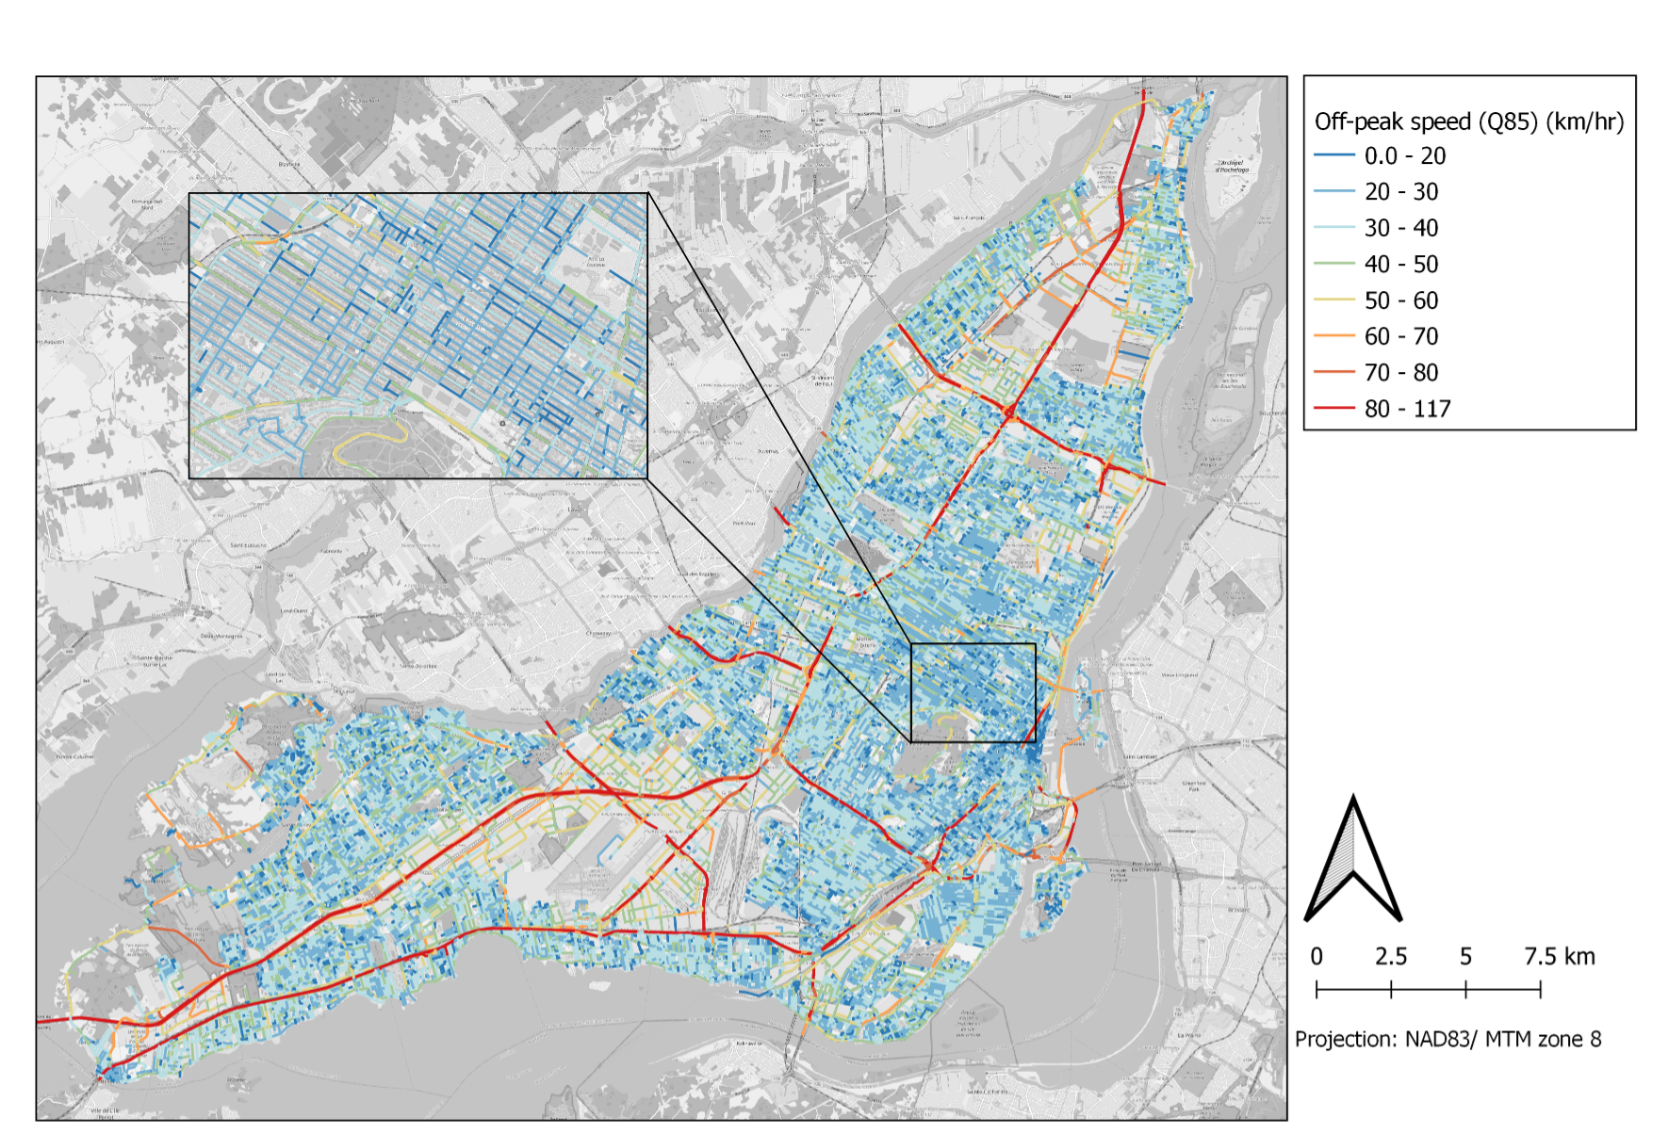
\includegraphics[width=\linewidth]{Figures/LTS_SpeedMeasures_link level.png}
        \caption{Off-peak 85th-percentile vehicle speeds.}
        \label{fig:lts_speed}
    \end{subfigure}
    \hfill
    \begin{subfigure}[t]{0.9\linewidth}
        \centering
        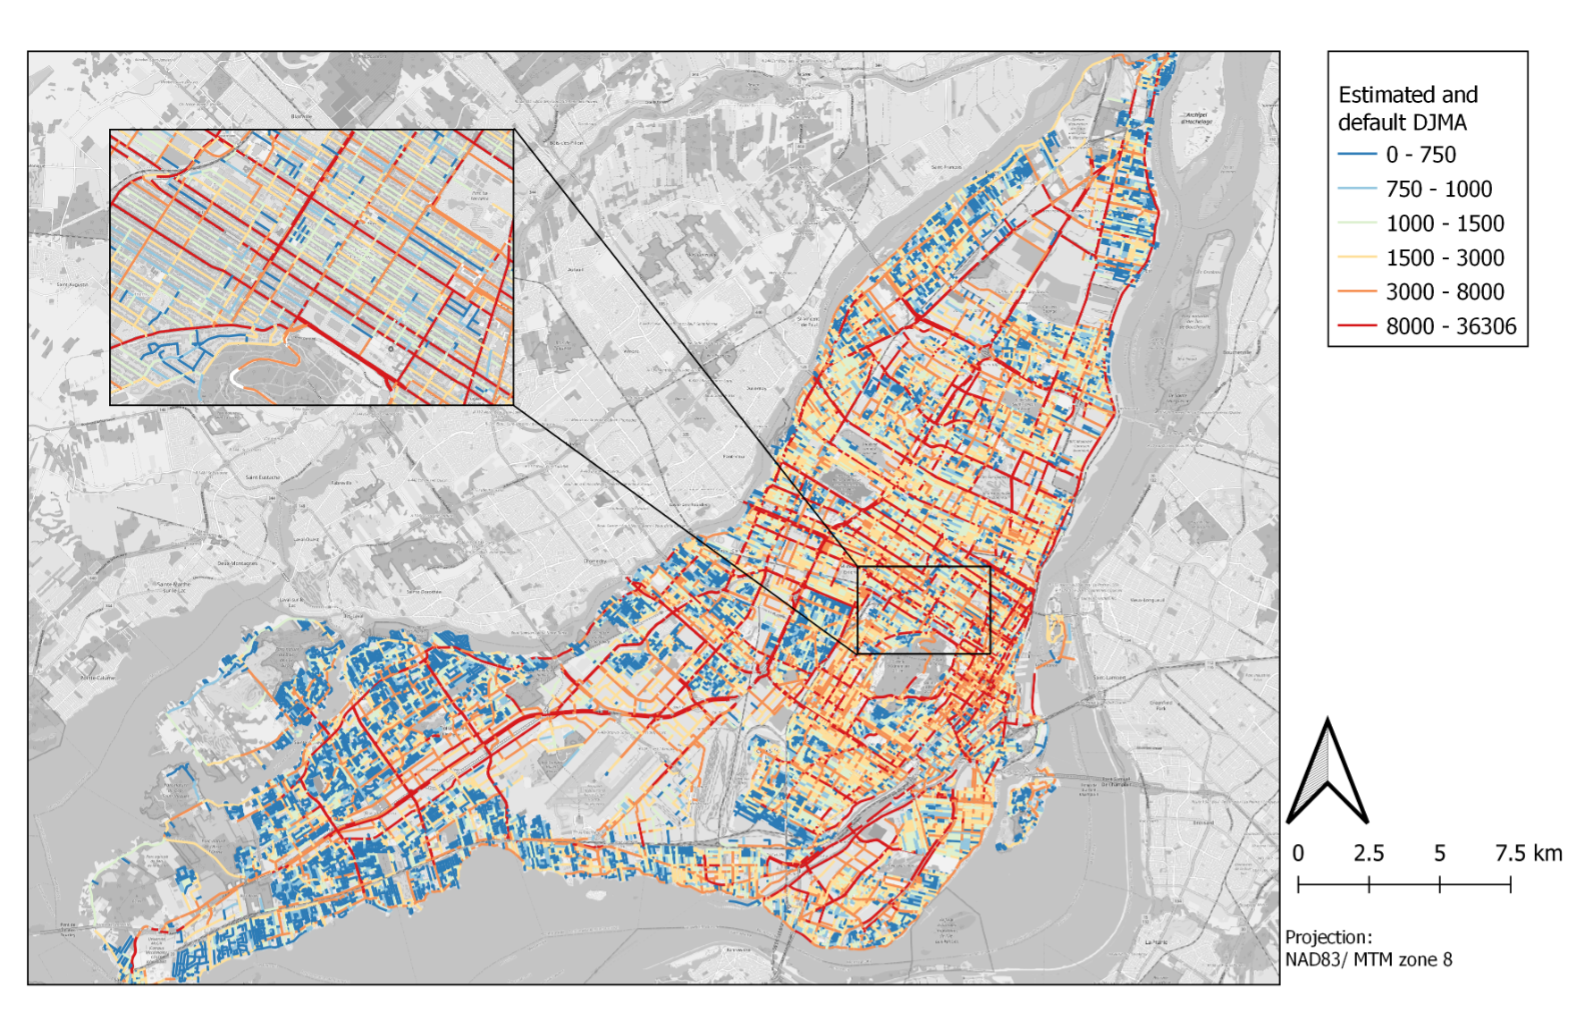
\includegraphics[width=\linewidth]{Figures/LTS_TrafficVolume_link level.png}
        \caption{Estimated traffic volume (ADT).}
        \label{fig:lts_traffic}
    \end{subfigure}
    \caption{Speed and volume distributions for Step 1: (a) off-peak vehicle speeds (85th-percentile) from GPS trajectories and (b) estimated traffic volumes (ADT) from regression models calibrated to observed traffic counts.}
    \label{fig:lts_measure_montreal}
\end{figure}
 
\textbf{Step 2 -- Infrastructure Validation and Refinement:} While speed and volume form the primary LTS classification inputs, bicycle infrastructure characteristics (lane width, continuity, separation from traffic, and centerline markings) also affect classification thresholds, particularly for painted bike lanes and mixed-traffic streets. Administrative datasets often encode these attributes inconsistently or incompletely. Rather than assuming the accuracy of administrative data, we conducted targeted validation using Google Maps satellite imagery. We identified segments that likely constitute classification exceptions (e.g., high-volume streets with newly constructed protective facilities or low-speed streets with inadequate infrastructure) and visually verified these critical segments. This strategic validation approach corrected the most consequential errors without requiring exhaustive inspection of every street, balancing accuracy against data-collection effort. We then consolidated all attributes (speed, volume, infrastructure, and geometric properties) into a unified geospatial database.
 
\textbf{Step 3 -- Automated LTS Classification:} In the final step, custom Python scripts applied LTS decision rules (Table~\ref{tab:lts_criteria}) to all network segments, using Montreal-specific parameters adapted from the LTS v2.0 framework. Automation ensures consistent application of classification logic across the entire network, eliminating manual inconsistencies and providing full transparency in decision-making. Each street segment is assigned a definitive LTS value, enabling its integration into the optimization model. 

\subsection{Multi-Objective Optimization Model and Mathematical Formulation}

This section outlines the mathematical formulation and algorithmic approach for solving the multi-objective MILP.
We detail the sets, indices, parameters, decision variables, and constraints that govern the optimization model.
Subsequently, we present the algorithm employed to derive optimal solutions, emphasizing practical applicability and transparency.

%\subsubsection{Mathematical Formulation}

The proposed formulation is a tri-objective MILP that supports coordinated planning of bikeway upgrades and station-based bike-sharing supply. The model operates on a candidate graph $G=(N,L)$, where nodes $i\in N$ represent candidate station locations and edges $(i,j)\in L$ represent candidate bikeway links that can be upgraded and included in the final network. The decision variables select which stations to activate ($y_i$), which links to include ($x_{ij}$), and how much capacity (e.g., docks) to allocate at each active station ($z_i$). The complete nomenclature of the model is presented in Table \ref{tab:notation}.

\begin{table}[!ht]
\caption{Notation and Definitions.}
\label{tab:notation}
\centering
\small
\begin{tabularx}{0.85\textwidth}{@{} l l X @{}}
\hline
\textbf{Category} & \textbf{Symbol} & \textbf{Definition} \\
\hline

\multicolumn{3}{l}{\textit{Sets and Indices}} \\
& $N$ & Set of candidate bicycle stations, indexed by $i,j \in N$. \\
& $L \subseteq N \times N$ & Set of candidate bicycle network links, indexed by $(i,j)\in L$. \\
\hline

\multicolumn{3}{l}{\textit{Parameters}} \\
& $D_i$ & Potential cycling demand associated with station $i$ [trips], $i\in N$. \\
& $D_i^{peak}$ & Daily peak-demand at station $i$ for docks sizing [trips], $i\in N$. \\
& $LTS_{ij}$ & Level of Traffic Stress on link $(i,j)$, $(i,j)\in L$. \\
& $C_{ij}^{up}$ & Upgrade investment for link $(i,j)$ [CAD\$], if selected. \\
& $C^{dock}$ & Unit cost of a dock [CAD\$/unit], $i\in N$. \\
& $D^{\min}$ & Minimum total demand to be covered [trips]. \\
& $S^{\min}$ & Minimum number of stations to activate. \\
& $M^{\min}$ & Minimum number of links to activate. \\
& $\alpha,\beta,\gamma$ & Weights used in the scalarized objective function. \\
\hline

\multicolumn{3}{l}{\textit{Decision Variables}} \\
& $x_{ij}\in\{0,1\}$ & 1 if link $(i,j)\in L$ is selected, 0 otherwise. \\
& $y_i\in\{0,1\}$ & 1 if station $i\in N$ is activated, 0 otherwise. \\
& $z_i \ge 0$ & Capacity allocated at station $i$ (number of docks), $i\in N$. \\
\hline
\end{tabularx}
\end{table}


\begin{align}
\label{obj1_new}
Z_1 &= \text{Maximize} \sum_{i \in N} D_i\, y_i \\
\label{obj2_new}
Z_2 &= \text{Minimize} \sum_{(i,j) \in L} LTS_{ij}\, x_{ij} \\
\label{obj3_new}
Z_3 &= \text{Minimize} \sum_{(i,j)\in L} C_{ij}^{up}\, x_{ij} \;+\; \sum_{i\in N} C^{dock}\, z_i
\end{align}

Three competing objectives are considered. The first objective $Z_1$ maximizes covered cycling demand by prioritizing activation of stations located in high-demand zones. The second objective $Z_2$ minimizes the total traffic stress exposure across the selected links using the LTS score as a proxy for perceived comfort and safety. The third objective, $Z_3$, captures investment requirements by combining link-upgrade and station-capacity costs. This explicitly accounts for the fact that achieving low-stress connectivity typically requires additional infrastructure investment, and that station deployments must be supported by adequate service capacity.

\begin{align}
\label{const2_new}
\sum_{i\in N} y_i &\ge S^{\min} \\
\label{const3_new}
\sum_{(i,j)\in L} x_{ij} &\ge M^{\min} \\
\label{const4_new}
\sum_{i\in N} D_i\, y_i &\ge D^{\min} \\
\label{const_cap}
z_i &\ge D_i^{peak}\, y_i \quad \forall i \in N \\
\label{const5_new}
x_{ij} &\le y_i \quad \forall (i,j)\in L \\
\label{const6_new}
x_{ij} &\le y_j \quad \forall (i,j)\in L \\
\label{const7_new}
y_k &\le \sum_{(i,j)\in L:\, i=k \text{ or } j=k} x_{ij} \quad \forall k\in N
\end{align}

The constraints enforce practical feasibility. Constraints \eqref{const2_new}--\eqref{const4_new} ensure that the solution meets minimum infrastructure and service requirements, namely a minimum number of activated stations, a minimum number of selected links, and a minimum level of covered demand. Constraint \eqref{const_cap} links station activation to a capacity requirement, forcing stations to be provisioned with sufficient docks (or capacity-units) to satisfy a peak demand proxy whenever they are selected. Constraints \eqref{const5_new} and \eqref{const6_new} enforce link--station consistency by preventing a link from being selected unless both of its endpoints are active. Finally, constraint \eqref{const7_new} prevents isolated stations by requiring that each active station be incident to at least one selected link, thereby promoting a connected, implementable design.

\subsection{Solution Algorithm}

To approximate the Pareto-efficient (non-dominated) set and make trade-offs among demand coverage, comfort, and cost explicit, we apply the Non-dominated Sorting Genetic Algorithm II (NSGA-II) \citep{debFastElitistMultiobjective2002}. NSGA-II is a well-established evolutionary multi-objective optimizer that uses elitist selection, non-dominated sorting, and crowding-distance ranking to preserve solution diversity along the Pareto front. An overview of the procedure applied in this paper is shown in Figure \ref{fig:solution_algorithm}.

\begin{figure}[htb]
\centering
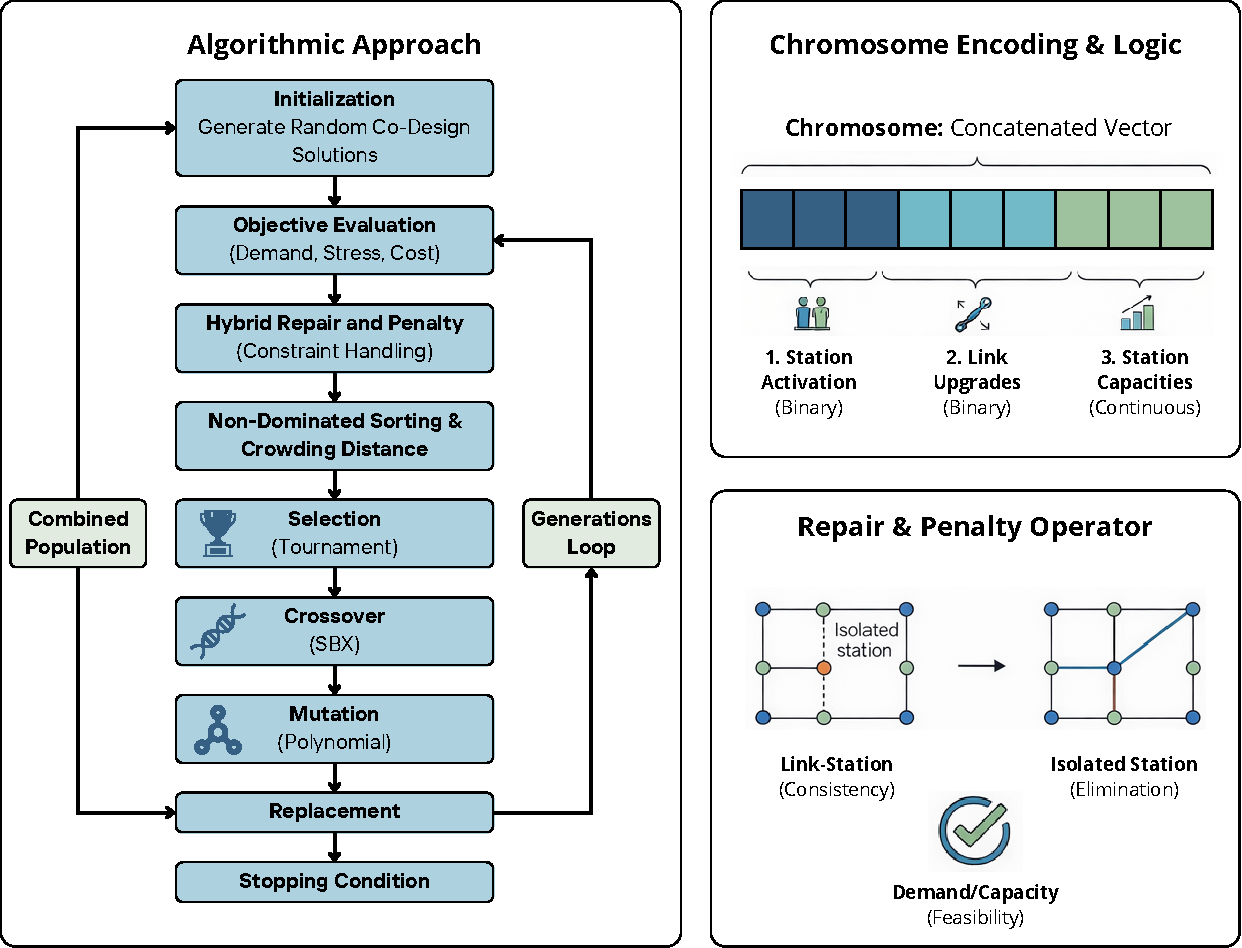
\includegraphics[width=1\textwidth]{Figures/ngsa_2.pdf}
\caption{Overview of the NSGA-II-based solution procedure for the integrated planning model.}
\label{fig:solution_algorithm}
\end{figure}

Given an initial population of candidate designs, NSGA-II iteratively improves solutions over generations using (i) objective evaluation, (ii) non-dominated sorting into Pareto fronts, (iii) diversity ranking via crowding distance, and (iv) variation operators (selection, crossover, mutation). At each generation, tournament selection favors solutions with better dominance rank and higher crowding distance. Offspring are generated through crossover and mutation, merged with the parent population, and then filtered via elitist replacement to form the next generation. The algorithm terminates after a predefined number of generations (or when improvement stagnates), returning a diverse approximation of the Pareto front that can be used to select representative designs for mapping and policy interpretation.

\textbf{Chromosome representation:} Each individual encodes a complete integrated plan with the same decision components as the MILP formulation: station activation, link selection for upgrade, and station capacity allocation. Specifically, the chromosome is defined as a concatenated vector:

\begin{equation}
\mathbf{g} \;=\; \big[\, \mathbf{y}\;|\;\mathbf{x}\;|\;\mathbf{z}\,\big],
\end{equation}

where $\mathbf{y}=\{y_i\}_{i\in N}$ are binary station activation variables, $\mathbf{x}=\{x_{ij}\}_{(i,j)\in L}$ are binary link selection variables, and $\mathbf{z}=\{z_i\}_{i\in N}$ are continuous nonnegative capacity variables. The chromosome dimension is therefore $2|N|+|L|$. This mixed encoding allows NSGA-II to explore joint decisions over network structure (stations and upgraded links) and operational feasibility (capacity) within a unified search space.

\textbf{Objective evaluation:} For each individual $\mathbf{g}$, objective values are computed using the definitions in Section~(ref). In particular, the algorithm evaluates (i) total covered demand induced by activated stations, (ii) total stress exposure over selected links based on $LTS_{ij}$, and (iii) total procurement cost combining link upgrade costs and station capacity costs. The resulting objective vector is used for Pareto dominance comparisons during non-dominated sorting:

\begin{equation}
\mathbf{Z}(\mathbf{g}) \;=\; \big(Z_1(\mathbf{g}),\, Z_2(\mathbf{g}),\, Z_3(\mathbf{g})\big)
\end{equation}



\textbf{Constraint handling and feasibility:} Variation operators can produce infeasible solutions that violate the logical and operational constraints of the planning problem. We handle feasibility using a hybrid approach consisting of (i) a repair operator and (ii) a penalty mechanism for any remaining violations. The repair operator enforces the key structural constraints used in the MILP: (a) link--station consistency (a link can only be selected if both endpoint stations are active), (b) prevention of isolated activated stations (each active station must be incident to at least one selected link), and (c) capacity feasibility (active stations must satisfy the peak-demand proxy through $z_i \ge D_i^{peak}y_i$). After repair, any residual violation is quantified through a scalar constraint-violation function $V(\mathbf{g})\ge 0$. During selection and sorting, infeasible solutions are penalized such that feasible solutions dominate infeasible ones, and among infeasible designs, lower violation is preferred. This strategy preserves the exploratory benefits of evolutionary search while steering the population toward implementable infrastructure plans.

\textbf{Variation operators:} We use operators that match the mixed decision structure. Two-point crossover is applied to the concatenated chromosome, preserving contiguous blocks of decisions. Mutation is applied using bit-flip operators for the binary components ($\mathbf{y}$ and $\mathbf{x}$) and Gaussian perturbation for the continuous component ($\mathbf{z}$), followed by nonnegativity bounding and repair. This design allows both structural modifications (adding/removing stations or upgrading links) and fine-grained adjustments (capacity reallocation) within the same evolutionary cycle.

\textbf{Parameter settings and termination:} NSGA-II performance depends on algorithm settings that control exploration, exploitation, and runtime. In the computational experiments, we specify a population size, number of generations, crossover probability, and mutation probabilities for both binary and continuous components. The algorithm terminates after a fixed number of generations, and the final output is the non-dominated set from the terminal population, which serves as an approximation of the Pareto front. We subsequently select representative solutions (e.g., demand-oriented, comfort-oriented, cost-oriented, and compromise designs) for visualization and planning interpretation.


% -------------------- Case Study --------------------


\section{Case Study Description}\label{casestudy}

Montreal offers an ideal setting for this study due to its large bike-sharing system and comprehensive data, which facilitate station and network optimization. The BIXI system records urban cycling demand, helping derive realistic station placement patterns. The street network includes various cycling facilities, allowing assessment of infrastructure comfort constraints on station configurations. This section details the demand patterns, candidate station location generation method, and the LTS mapping and parameters used in experiments.

\subsection{BIXI Demand Patterns and Candidate Station Locations}\label{subsec:bixi_demand}

The processed 2025 BIXI dataset includes 14,249,363 trips across 1,296 origin stations, providing a detailed empirical representation of urban cycling demand. Key summary statistics are reported in Table \ref{tab:bixi_data_summary}.

\begin{table}[htbp]
  \centering
  \caption{Summary statistics of the 2025 BIXI dataset used in this case study.}
  \label{tab:bixi_data_summary}
  \small
  \begin{tabularx}{0.82\textwidth}{@{} l X @{} }
    \hline
    \textbf{Indicator} & \textbf{Value} \\
    \hline
    Annual BIXI trips (2025) & 14,249,363 \\
    Distinct origin stations & 1,296 \\
    Share of origins in Le Plateau-Mont-Royal and Ville-Marie & 57.5\% \\
    Activity captured by top 30 stations & 3,508,845 trips \\
    Activity captured by top 10 stations & 1,553,726 trips \\
    Trips occurring from April to November & 97.6\% \\
    Trips occurring from June to September & 63.7\% \\
    \hline
  \end{tabularx}
\end{table}

Two structural features are particularly relevant for the optimization problem. First, demand is strongly centralized, with Le Plateau-Mont-Royal and Ville-Marie accounting for 57.5\% of trip origins, indicating a well-defined high-activity corridor. Second, usage is highly seasonal, with 97.6\% of trips occurring between April and November and 63.7\% during June to September, reflecting Montreal’s climatic constraints.

To focus the analysis on the most critical trade-offs between coverage, comfort, and investment, we consider the 30 highest-activity stations within the downtown cluster (Figure \ref{fig:bixi_demand_map}). These stations account for 3.51 million interactions, with the top 10 alone contributing 1.55 million, ensuring that the study area captures the most intensive portion of system demand. The full list of selected stations and their activity levels is provided in \ref{app:top30_stations}.

\begin{figure}[htbp]
    \centering
    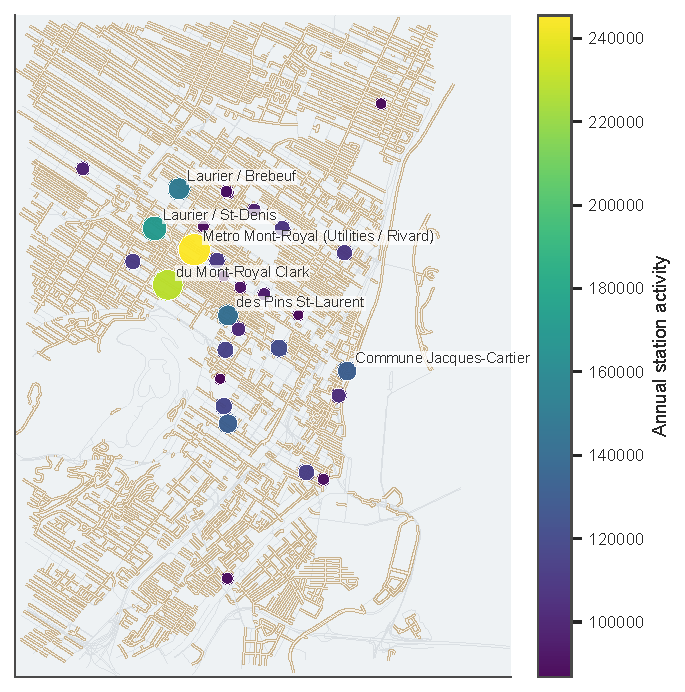
\includegraphics[width=0.72\textwidth]{Figures/BIXI_case_top30_station_map.pdf}
    \caption{Spatial distribution of the 30 highest-activity BIXI stations within the downtown study area.}
    \label{fig:bixi_demand_map}
\end{figure}

At a broader spatial scale, demand also clusters at the borough level. Figure~\ref{fig:bixi_borough_activity} shows origin and destination volumes across Montreal’s main boroughs. Le Plateau-Mont-Royal, Ville-Marie, and Rosemont--La Petite-Patrie dominate both, while neighboring boroughs exhibit directional imbalances. This pattern indicates that the downtown core operates as part of a larger central activity belt rather than an isolated demand center.

\begin{figure}[htbp]
    \centering
    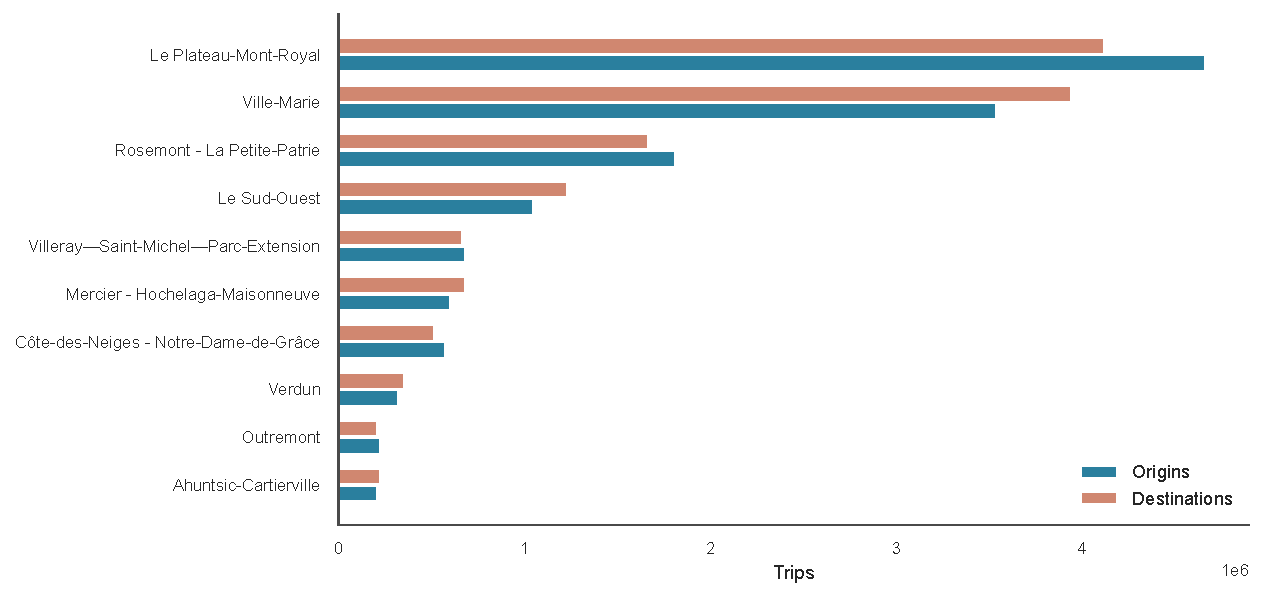
\includegraphics[width=0.80\textwidth]{Figures/BIXI_case_borough_activity.pdf}
    \caption{Origin and destination activity volumes across Montreal's boroughs.}
    \label{fig:bixi_borough_activity}
\end{figure}

\subsubsection{Temporal Demand Structure}

Beyond spatial patterns, BIXI demand exhibits strong temporal variation at multiple timescales. Understanding this temporal structure is essential for calibrating demand assumptions in the optimization model. Figure~\ref{fig:bixi_temporal_ab} shows complementary perspectives on demand timing at different temporal scales.

\begin{figure}[htbp]
    \centering
    \begin{subfigure}[t]{0.8\textwidth}
        \centering
        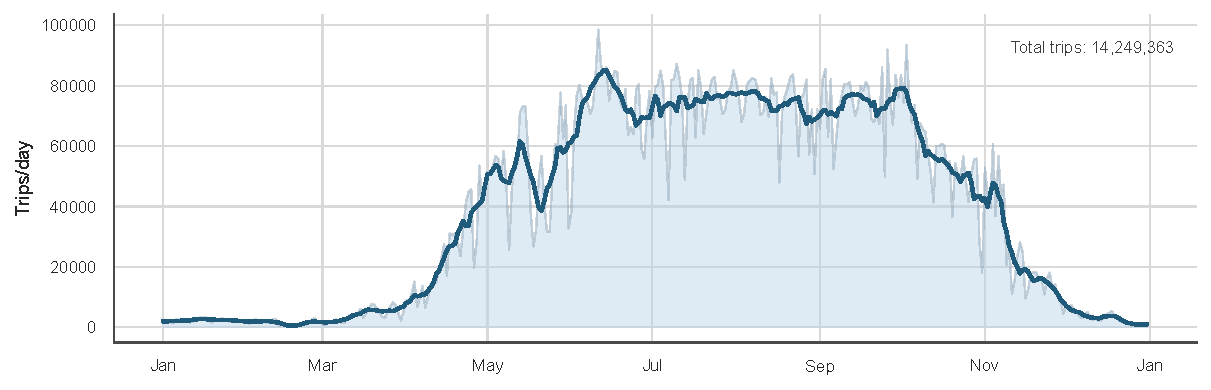
\includegraphics[width=\linewidth]{Figures/BIXI_case_daily_ridership.pdf}
        \caption{Daily ridership profile.}
        \label{fig:bixi_daily_profile}
    \end{subfigure}
    
    \vspace{0.4cm}
    
    \begin{subfigure}[t]{0.8\textwidth}
        \centering
        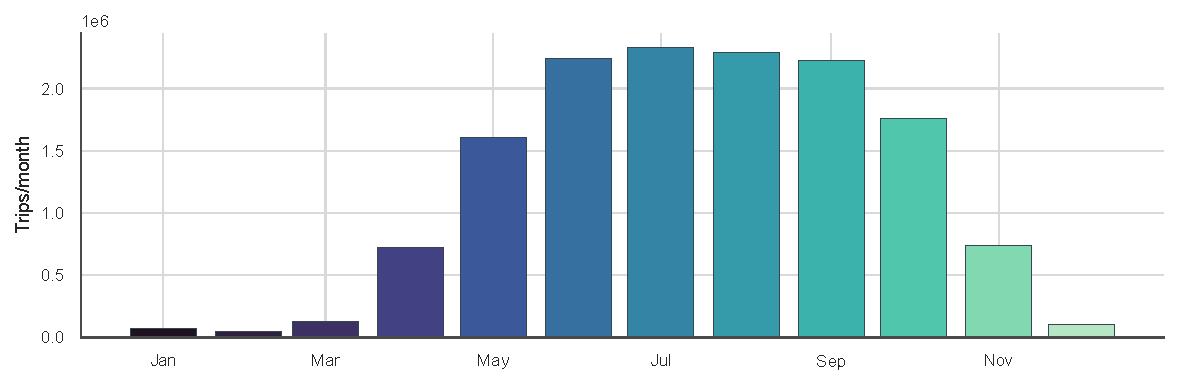
\includegraphics[width=\linewidth]{Figures/BIXI_case_monthly_ridership.pdf}
        \caption{Monthly ridership profile.}
        \label{fig:bixi_temporal_patterns}
    \end{subfigure}
    
    \caption{Temporal evolution of BIXI ridership in 2025 across (a) daily and (b) monthly scales.}
    \label{fig:bixi_temporal_ab}
\end{figure}

At the seasonal scale (Figure~\ref{fig:bixi_daily_profile}), ridership follows a pronounced annual cycle characterized by a rapid ramp-up beginning in spring, a sustained plateau during summer months, and a marked decline as fall arrives. This seasonality reflects Montreal's winter climate and demonstrates that BIXI functions primarily as a warm-season mobility option. At the sub-annual scale (Figure~\ref{fig:bixi_temporal_patterns}), ridership peaks in the months of June through September, which account for 63.7\% of annual trips. This concentration has important implications for planning: it suggests that infrastructure investments and station placement should prioritize serving peak-season demand, while recognizing that the system experiences reduced but non-trivial activity during shoulder months.

Figure~\ref{fig:bixi_weekly_profile} presents a heatmap of BIXI departures by day of week and hour of day, revealing a distinct weekly structure.

\begin{figure}[htbp]
    \centering
    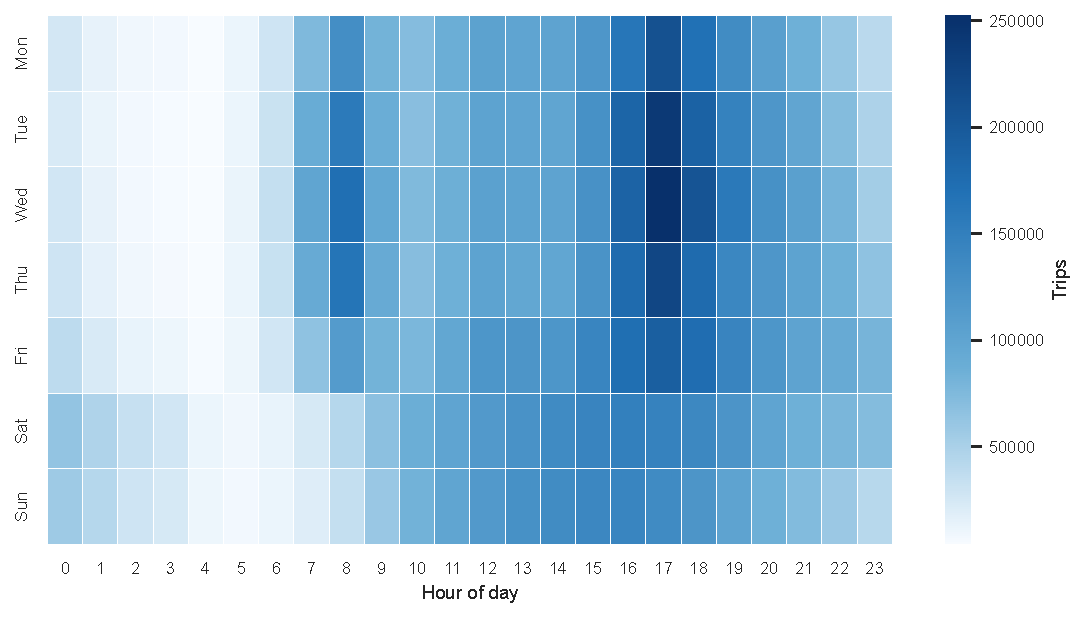
\includegraphics[width=0.75\textwidth]{Figures/BIXI_case_weekday_hour_heatmap.pdf}
    \caption{Weekly and hourly usage structure of BIXI departures in 2025.}
    \label{fig:bixi_weekly_profile}
\end{figure}

In the optimization framework, we use annual observed origin-destination demand as the planning baseline. This approach captures the full diversity of demand patterns while allowing the algorithm to identify station configurations that perform well across multiple temporal windows. The temporal concentrations documented above inform our interpretation of optimization results, allowing us to assess whether solutions prioritize peak-season performance or balance demand across seasons.

\subsubsection{Candidate Station Location Generation}

To allow station placement decisions to respond to comfort constraints, we generate multiple candidate locations for each existing station. For each of the 30 high-activity stations, we define a service buffer around the current location and generate five equidistant candidate sites within this buffer. This approach enables the optimization model to either retain an existing station's current location or relocate it to a nearby alternative site if doing so improves access to low-stress cycling infrastructure. For example, if a station's current location requires access via high-stress network segments, the algorithm may select an alternative candidate location that provides better integration with comfortable, low-stress facilities.

\subsection{Cycling Comfort and LTS Mapping}\label{subsec:lts_mapping}

Figure~\ref{fig:lts_mapping} visualizes the spatial distribution of LTS classifications across Montreal. 

\begin{figure}[htbp]
    \centering
    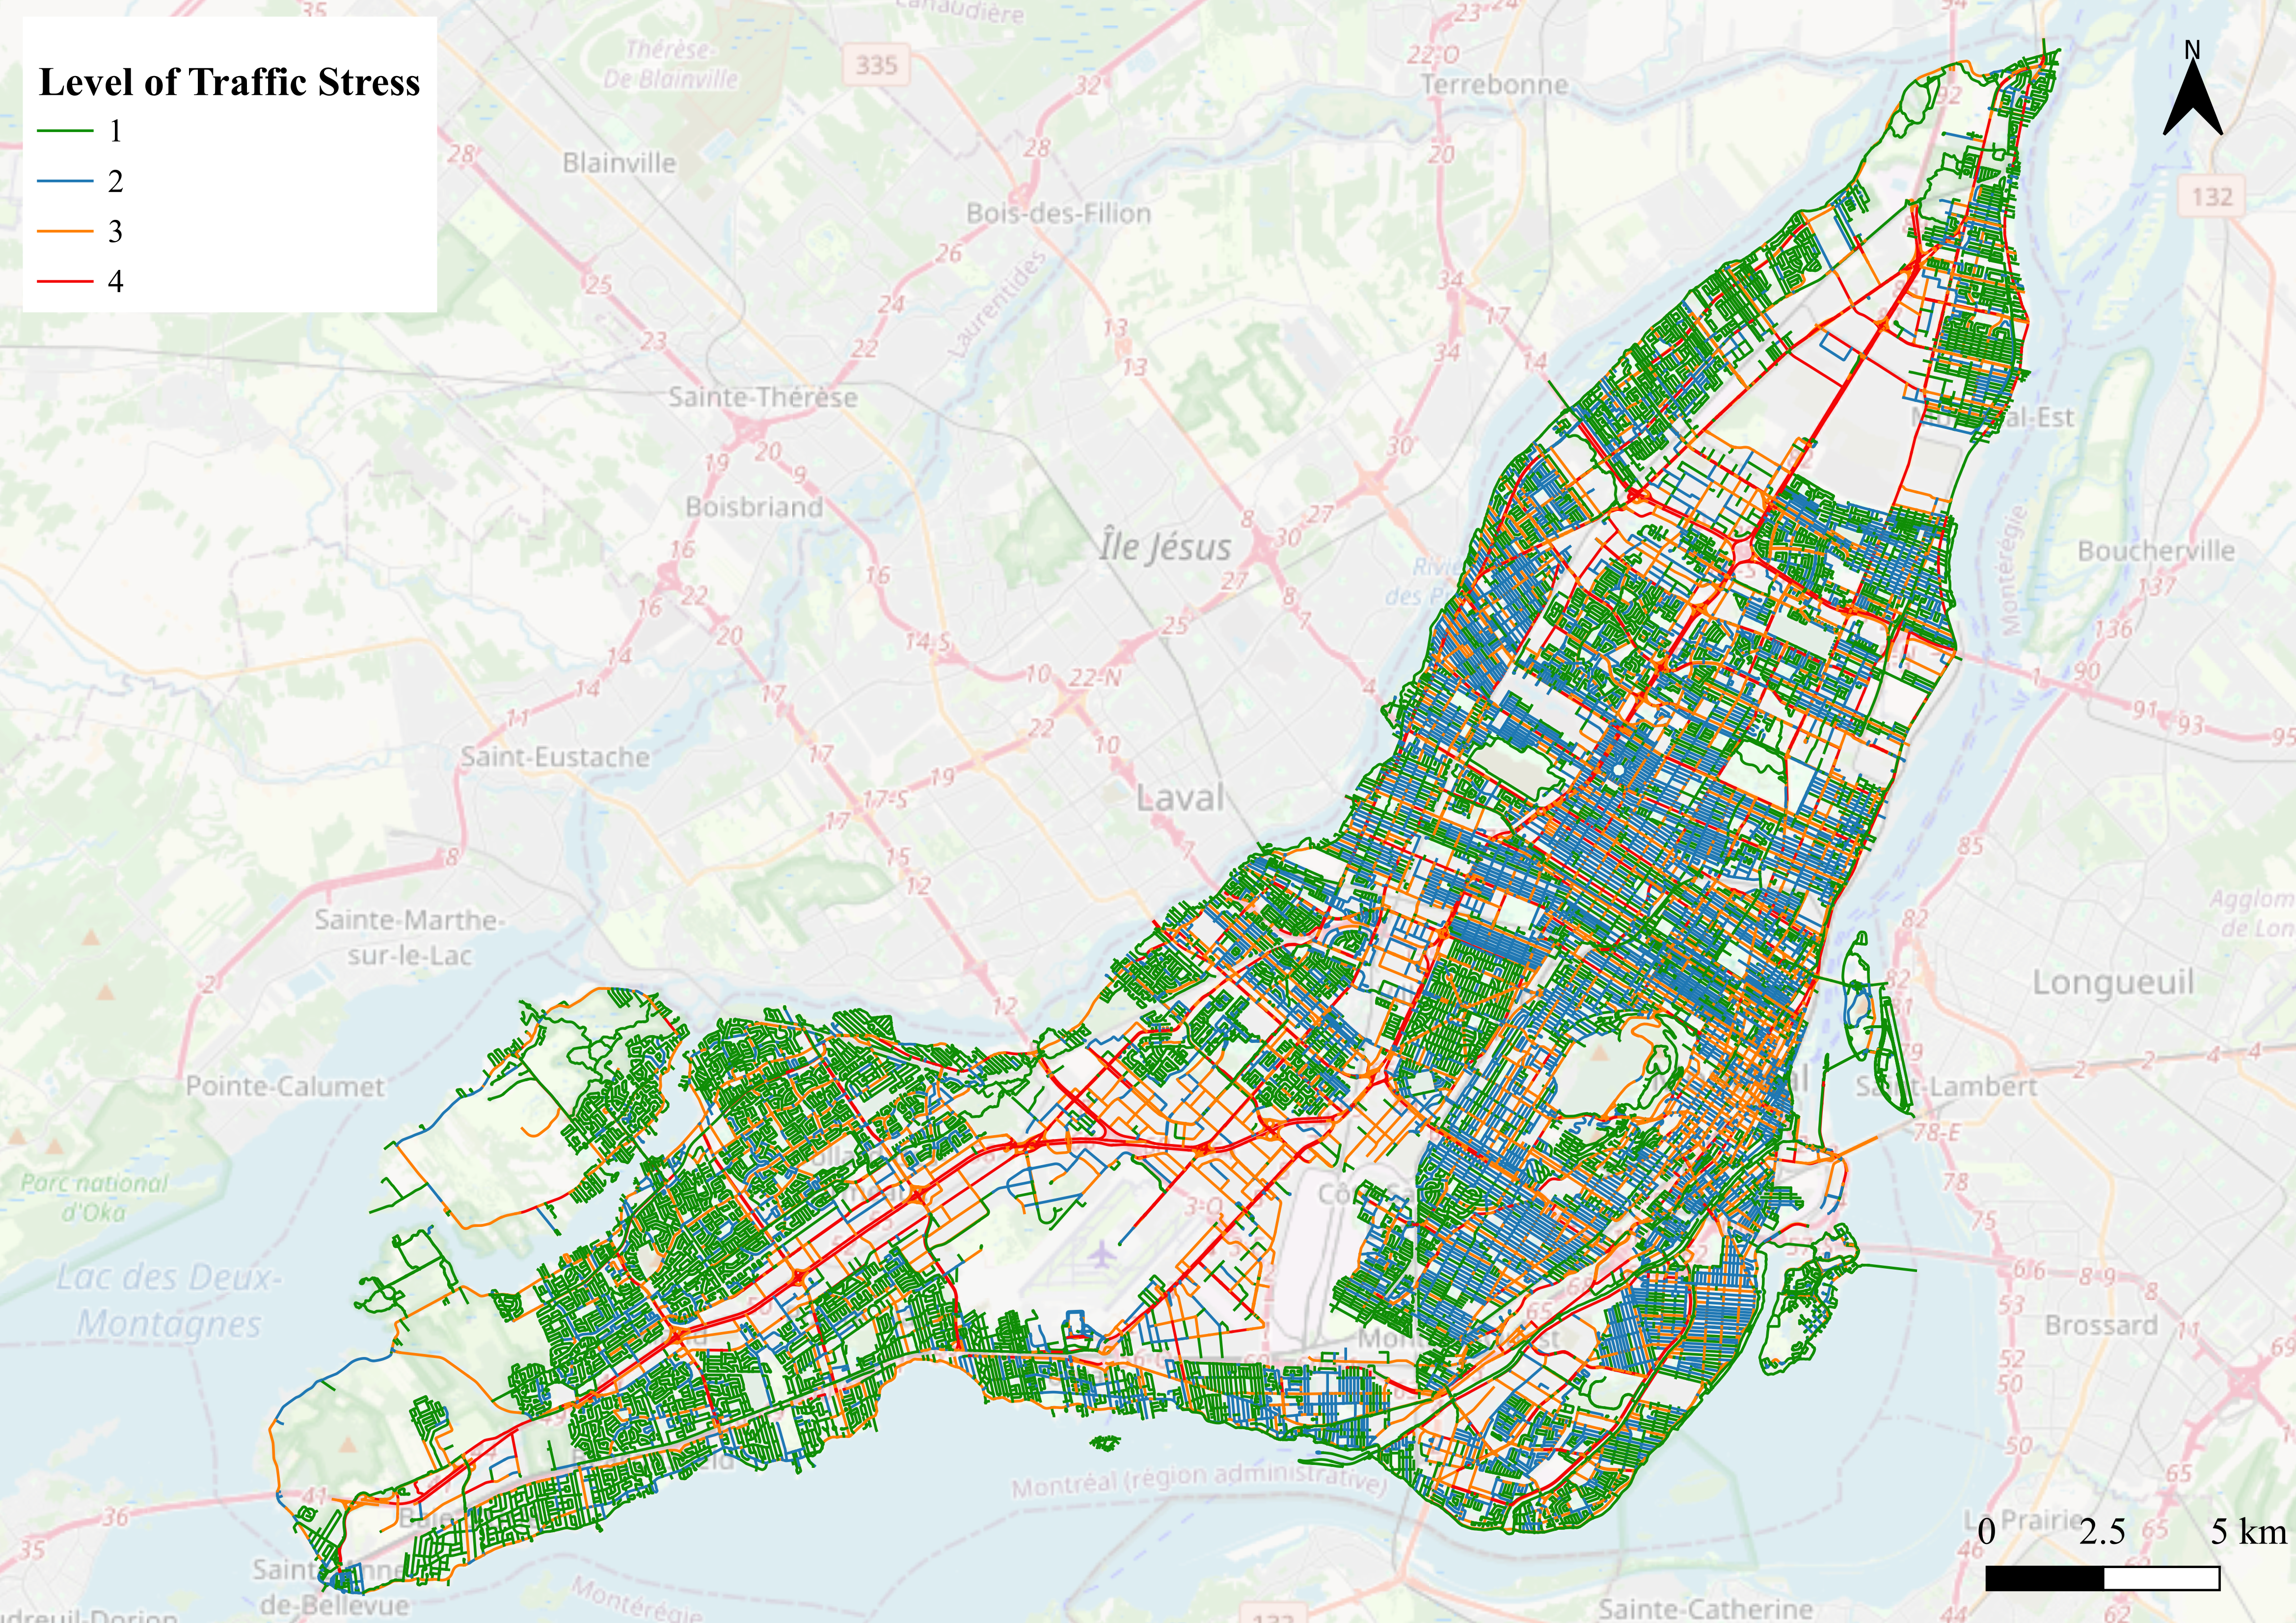
\includegraphics[width=0.7\textwidth]{Figures/LTS_Mapping2.png}
    \caption{Spatial distribution of LTS levels across Montreal's street network.}
    \label{fig:lts_mapping}
\end{figure}

Low-stress facilities (LTS 1--2) are more prevalent in central neighborhoods where cycling infrastructure is relatively dense and well-connected. However, many arterial corridors and major intersections remain classified as high-stress (LTS 3--4), and these high-stress segments often function as network bottlenecks. Even when local low-stress facilities exist, high-stress bottlenecks can dramatically reduce end-to-end network usability by forcing users to traverse uncomfortable or potentially unsafe conditions. This topology has important implications for station placement: locating a station to require access via high-stress links makes it less attractive regardless of its accessibility to local demand concentrations.

In the optimization model, LTS serves two complementary roles. First, it characterizes the comfort and perceived safety of the cycling network. Second, it guides investment decisions by identifying priority corridors for infrastructure improvement. When the algorithm selects a link for upgrade, it is assumed to improve that link to a low-stress standard (LTS 1), with costs specified as a function of the link's initial category. This framework ensures that optimization solutions account for both the current state of the network and the feasible improvements that can be made within budget constraints.

\subsection{Optimization Parameters and Algorithm Settings}\label{subsec:parameters}

The optimization model requires specification of both planning parameters (costs, service requirements) and algorithmic hyperparameters (population size, convergence settings). First, the planning parameters are specified in Table \ref{tab:global_parameters}.

\begin{table}[htbp]
  \caption{Economic and service parameters applied in the station and network optimization model.}
  \label{tab:global_parameters}
  \centering
  \small
  \setlength{\tabcolsep}{6pt}
  \renewcommand{\arraystretch}{1.15}
  \begin{tabularx}{0.85\textwidth}{@{} l X @{}}
    \hline
    \textbf{Parameter} & \textbf{Value} \\\hline
    Dock (capacity-unit) cost, $C_i^{\text{dock}}$ & 500 [CAD\$/unit] \\
    Minimum total demand covered, $D_{\min}$ & 150,000 [trips] \\
    Minimum number of stations, $S_{\min}$ & 30 [stations] \\
    Minimum number of links, $M_{\min}$ & 50 [links] \\
    Link upgrade cost, $C_{ij}^{\text{up}}$ & $\{0; 5{,}000; 10{,}000; 50{,}000\}$ [CAD\$] \\
    & for $\text{LTS}_{ij}=\{1,2,3,4\}$ \\
    \hline
  \end{tabularx}
\end{table}

Cost inputs follow values reported in prior planning studies and system evaluations. Dock costs reflect typical capital expenditures for bike-sharing capacity, while link upgrade costs vary by LTS category, with low-stress facility upgrades commanding higher investment than basic improvements. Links initially classified as LTS 1 require no upgrade and incur zero cost. Minimum service requirements (demand coverage, station count, link count) are specified to prevent degenerate solutions that would be unsuitable for practical planning. Demand and capacity parameters are derived directly from the processed BIXI origin-destination dataset.

Further, Table~\ref{tab:nsga2_hyperparams} presents the baseline NSGA-II settings applied throughout the computational experiments. 

\begin{table}[htbp]
  \centering
  \caption{NSGA-II hyperparameters.}
  \label{tab:nsga2_hyperparams}
  \small
  \renewcommand{\arraystretch}{1.15}
  \begin{tabular}{l @{\hspace{2.0cm}} r}
    \hline
    \textbf{Algorithm Parameter} & \textbf{Value} \\
    \hline
    Crossover probability & 0.90 \\
    Mutation probability & 0.20 \\
    Tournament size & 2 \\
    Initial population size & 3,000 \\
    Number of objectives & 3 \\
    Number of generations & 100 \\
    \hline
  \end{tabular}
\end{table}

These hyperparameters were held constant across all scenarios to ensure that resulting Pareto fronts are directly comparable and that differences in optimization outcomes reflect differences in planning objectives and constraints rather than variations in algorithm configuration.


% -------------------- Results --------------------
\section{Results and Discussion}\label{results}

This section presents results obtained by applying the proposed tri-objective model to the Montreal case study. Because the problem involves competing goals, maximizing demand coverage (Z1), minimizing cyclist stress exposure (Z2), and minimizing investment cost (Z3), the solutions are analyzed in terms of Pareto efficiency. First, the geometry of the approximated Pareto set in objective space is examined, and then planning implications through representative designs mapped onto the study area are interpreted. Finally, the model's robustness is evaluated by re-running the search with alternative constraint thresholds and assessing how the attainable trade-off surface shifts as requirements tighten.


\subsection{Pareto Front Approximation}

The NSGA-II algorithm generates an approximation of the Pareto frontier that captures trade-offs among demand coverage, cyclist stress exposure, and investment cost. Figure~\ref{fig:pareto_2d} presents pairwise projections of the final population in objective space.

\begin{figure}[htbp]
  \centering
  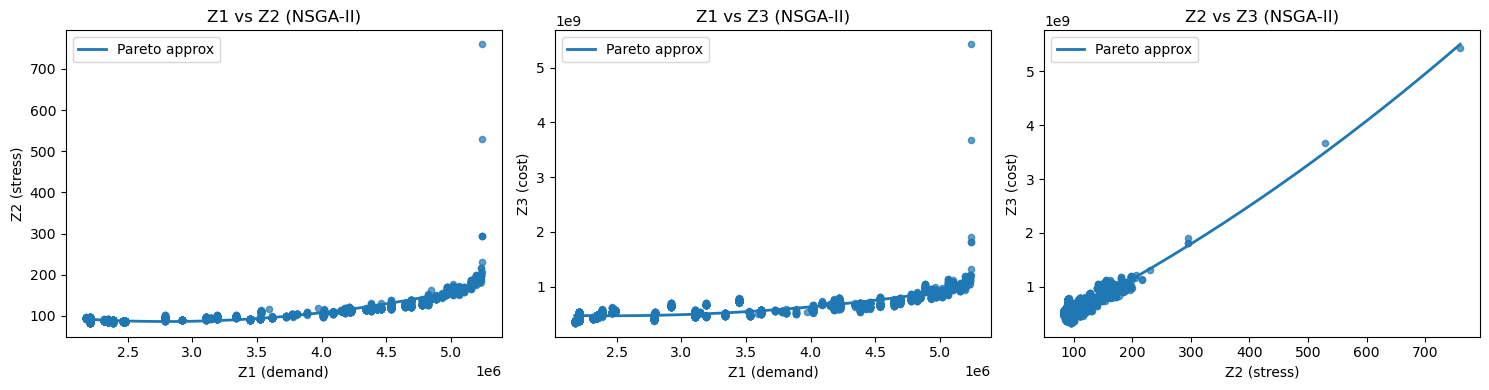
\includegraphics[width=\textwidth]{Figures/Plots_2D_Pop_3000_Gen_100.png}
  \caption{Pairwise projections of the NSGA-II Pareto set showing trade-offs among demand coverage, LTS, and investment cost.}
  \label{fig:pareto_2d}
\end{figure}


The distributions indicate a clear trade-off structure, showing that increasing covered demand typically requires either additional infrastructure upgrades or capacity provisioning, which raises investment costs and may expose more links to higher-stress conditions, reflecting the inherent tension among coverage expansion, comfort, and cost. The $Z_2$–$Z_3$ projection further indicates a strongly increasing, nonlinear relationship, suggesting that reductions in stress are typically achieved through disproportionate increases in upgrade costs. Figure~\ref{fig:pareto_3d} provides the corresponding three-dimensional view of the Pareto set. 

\begin{figure}[htb]
  \centering
  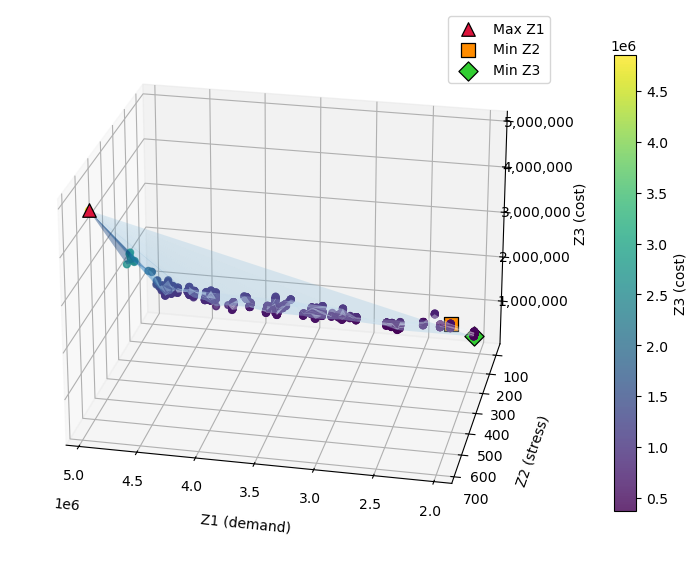
\includegraphics[width=0.65\textwidth]{Figures/Plots_3D_Pop_3000_Gen_100.png}
  \caption{Three-dimensional visualization of the NSGA-II Pareto set in $(Z_1, Z_2, Z_3)$ space, illustrating the structured trade-off surface between coverage, comfort, and cost.}
  \label{fig:pareto_3d}
\end{figure}

The plot shows that non-dominated solutions lie along a structured manifold, revealing a limited number of policy-relevant compromise regions (e.g., moderate coverage with moderate stress and cost versus high-coverage solutions with sharply increased stress and cost). This structure supports the selection of a small set of representative designs for mapping and interpretation in the next section.

\subsection{Analysis of Selected Pareto-Optimal Solutions}

To support interpretation and policy relevance, four representative solutions were extracted and visualized: \textit{Best Demand}, \textit{Best Stress}, \textit{Best Cost}, and a \textit{Balanced solution}. Table \ref{tab:nsga_solutions_size} summarizes the network size of the four representative solutions by reporting the number of selected stations and links in each configuration.

\begin{table}[htbp]
  \caption{Summary of representative NSGA-II solutions and selected network size.}
  \label{tab:nsga_solutions_size}
  \centering
  \small
  \begin{tabular}{@{}lccccc@{}}
    \hline
    \textbf{Solution} & \textbf{Selected Stations} & \textbf{Selected Links} & \textbf{Z1 (million)} & \textbf{Z2} & \textbf{Z3 (million)} \\
    \hline
    Best Demand  & 100 & 343 & 4.902 & 685.62 & 48.5 \\
    Best Stress  & 44  & 50  & 2.277 & 81.93  & 5.60 \\
    Best Cost    & 46  & 50  & 2.059 & 90.74  & 3.76 \\
    Balanced     & 93  & 72  & 4.613 & 138.53 & 9.42 \\
    \hline
  \end{tabular}
\end{table}

The \textit{Best Demand} solution activates the largest number of stations (100) and links (343), achieving the highest coverage (4.90 million trips), but at the expense of substantially higher stress and cost. In contrast, the \textit{Best Stress} and \textit{Best Cost} solutions produce much more compact networks, each with around 50 links and fewer than 50 stations, reducing stress and investment but covering only about half of the demand.  The \textit{Balanced solution} provides a more efficient compromise. With 93 stations and only 72 links, it achieves near-maximum demand coverage (4.61 million trips) while significantly reducing both stress and cost relative to the demand-oriented extreme. This indicates that most high-demand areas can be effectively served without requiring a fully dense network, provided that key connections are strategically selected. To deepen the analysis, Figure \ref{fig:Map_comparison} compares the corresponding spatial network configurations (selected stations and upgraded links) for these four solutions.

\begin{figure}[htbp]
    \centering
    \begin{subfigure}[b]{0.48\textwidth}
        \centering
        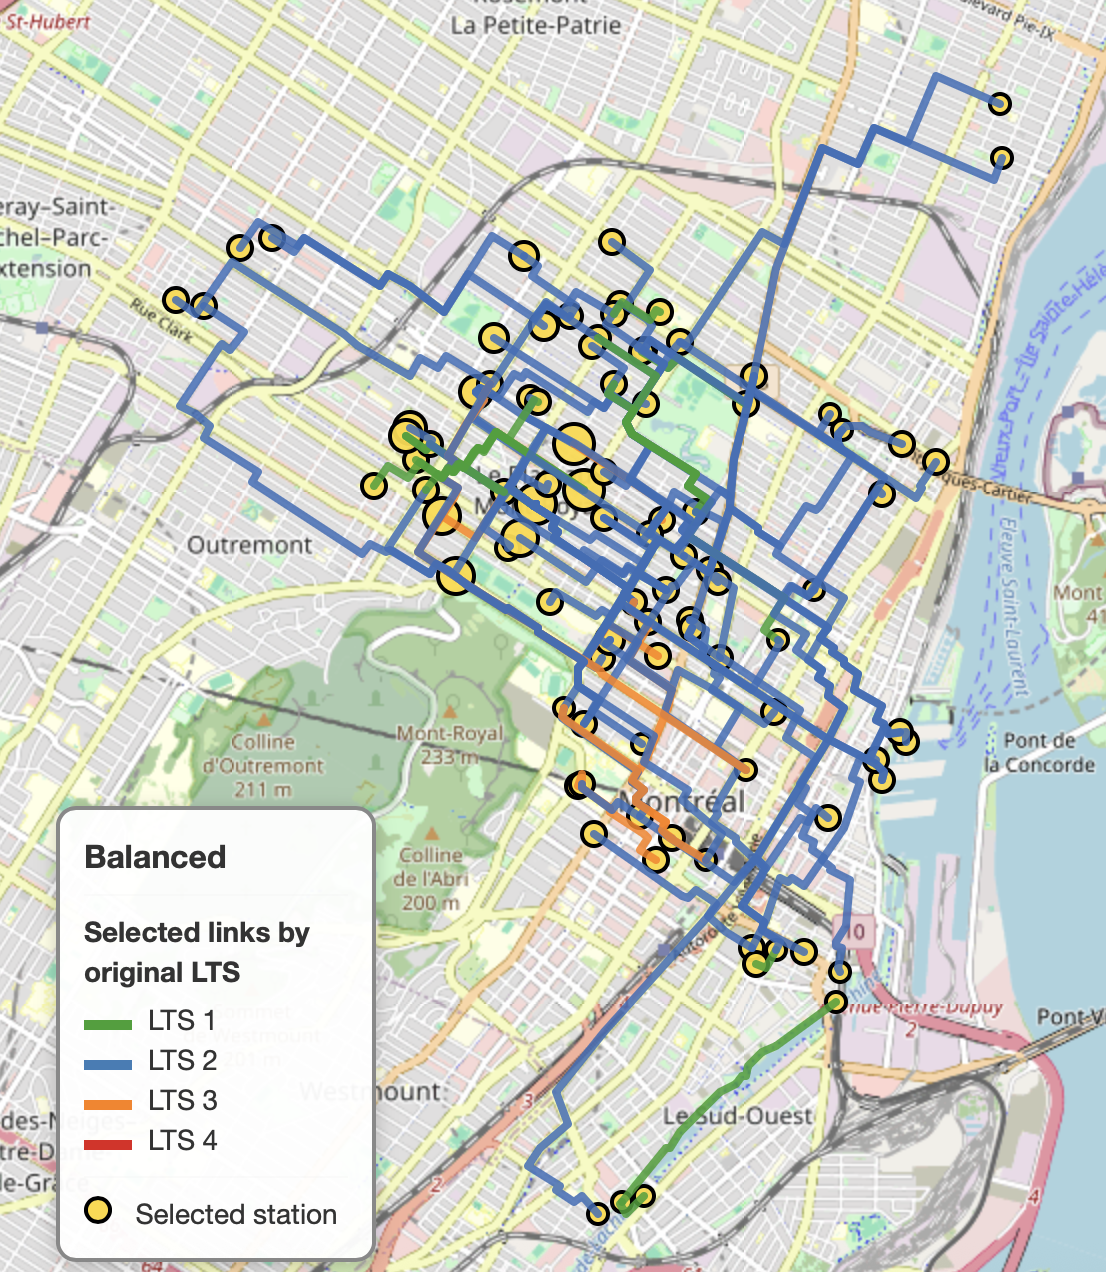
\includegraphics[width=\textwidth]{Figures/nsga_Balanced_Solution_map_3000_100.png}
        \caption{Balanced Solution.}
        \label{fig:Balanced_Solution}
    \end{subfigure}
    \hfill
    \begin{subfigure}[b]{0.48\textwidth}
        \centering
        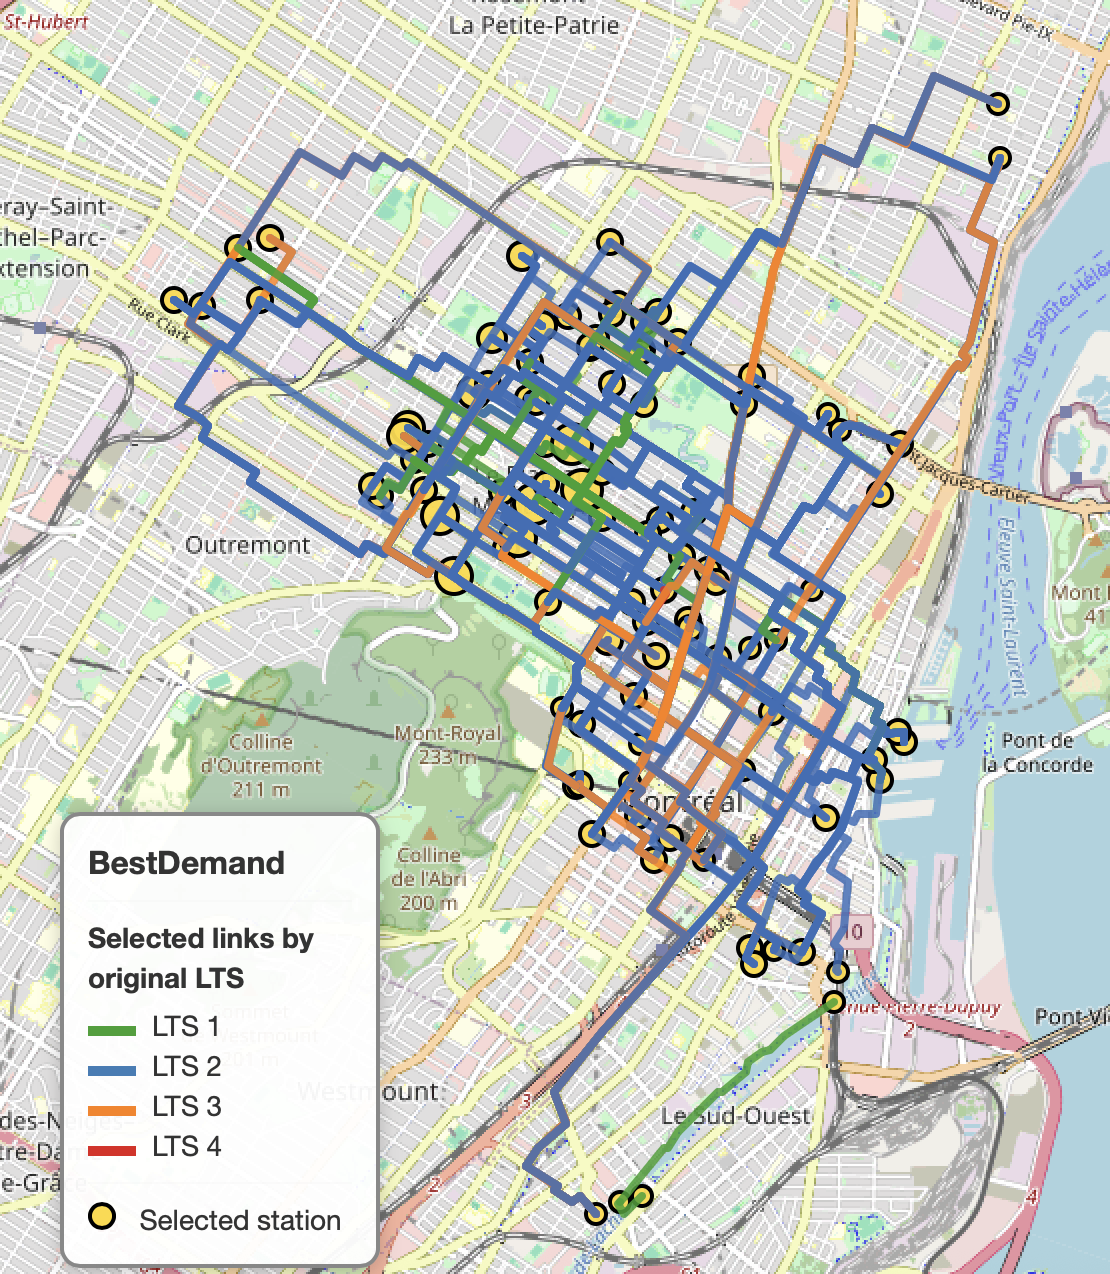
\includegraphics[width=\textwidth]{Figures/nsga_Best_Demand_map_3000_100.png}
        \caption{Best demand solution.}
        \label{fig:Best_Demand}
    \end{subfigure}
    
 \vspace{0.5cm}
    \begin{subfigure}[b]{0.48\textwidth}
        \centering
        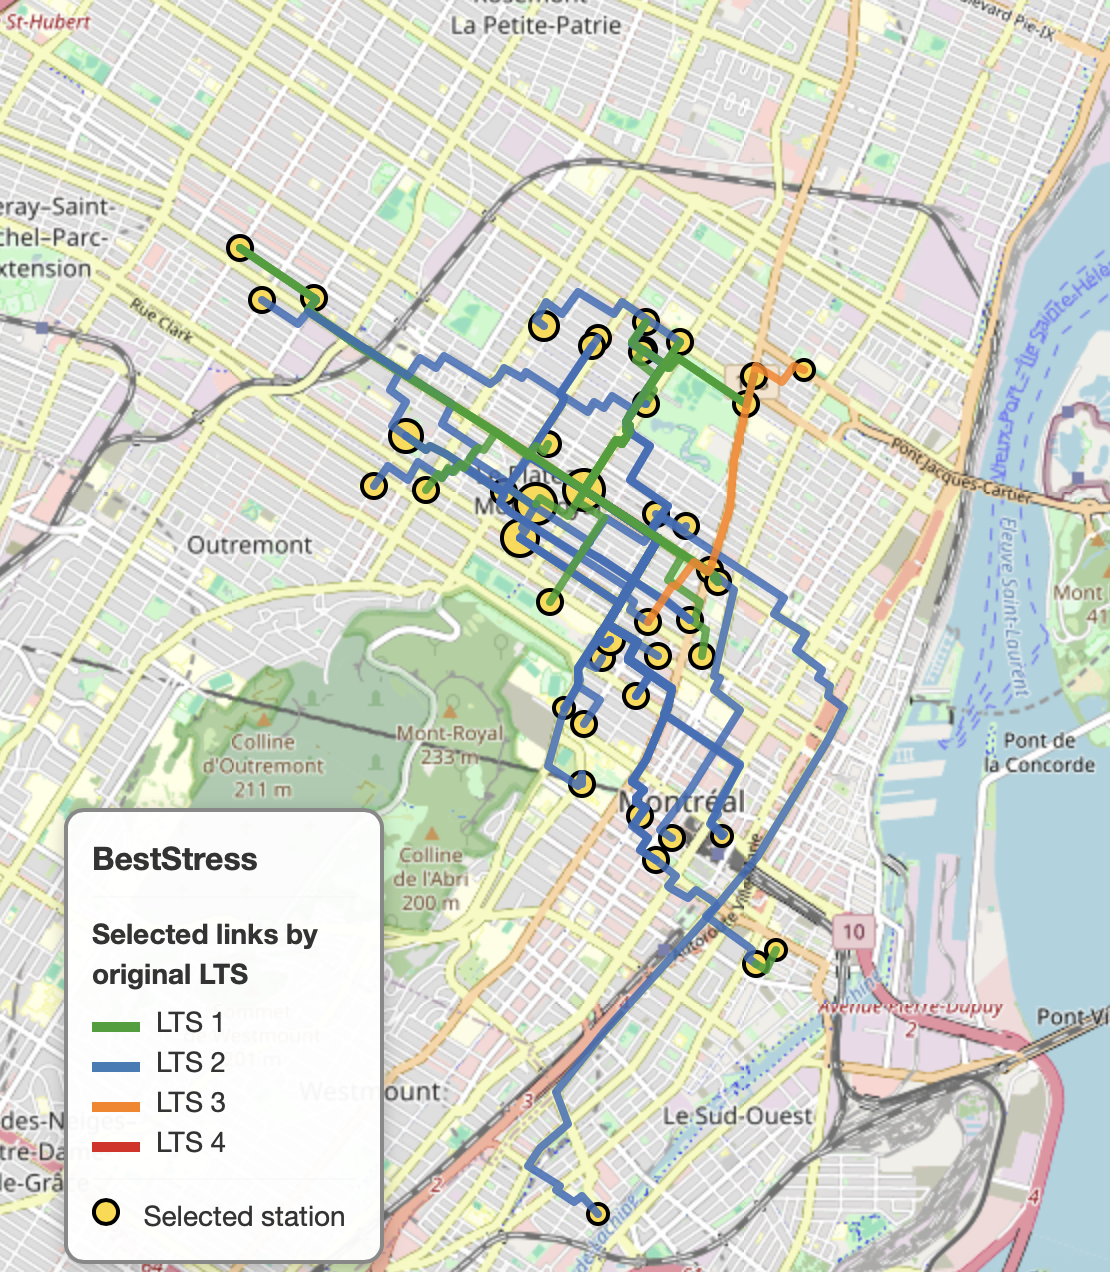
\includegraphics[width=\textwidth]{Figures/nsga_Best_Stress_map_3000_100.png}
        \caption{Best Stress Solution.}
        \label{fig:Best_Stress}
    \end{subfigure}
    \hfill
    \begin{subfigure}[b]{0.48\textwidth}
        \centering
        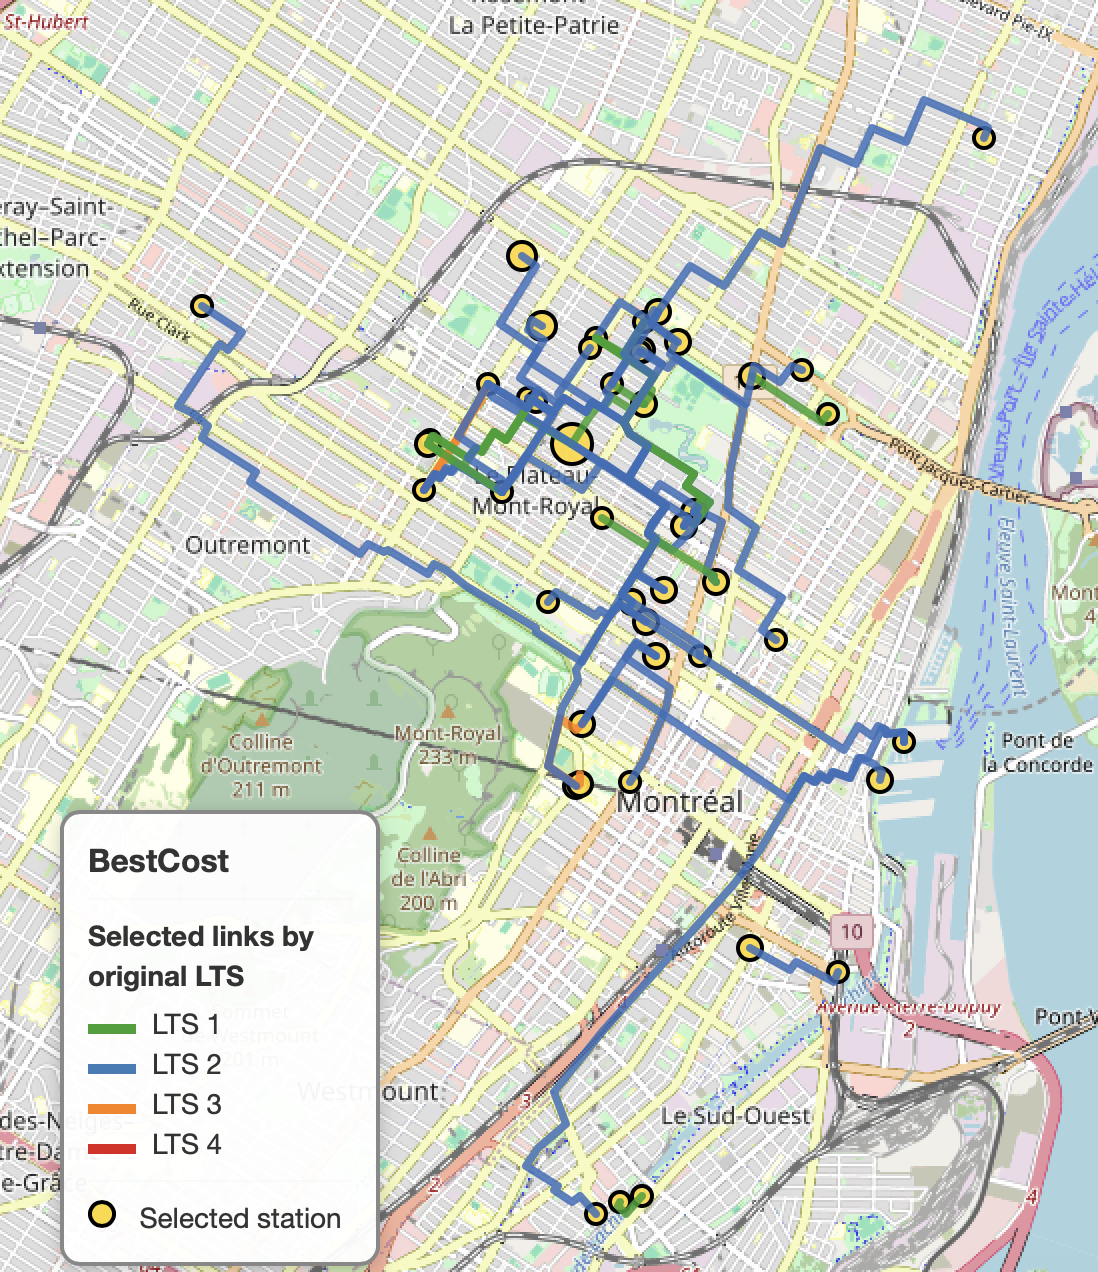
\includegraphics[width=\textwidth]{Figures/nsga_Best_Cost_map_3000_100.png}
        \caption{Best cost solution.}
        \label{fig:Best_Cost}
    \end{subfigure}
    \caption{Network configuration comparison of four representative Pareto-optimal solutions, illustrating distinct planning trade-offs between coverage, comfort, and cost.}
    \label{fig:Map_comparison}
\end{figure}

The network maps highlight clear spatial trade-offs between coverage, comfort, and investment. The \textit{Best Demand} solution concentrates infrastructure along major activity corridors, producing a dense network that maximizes coverage but requires extensive upgrades and higher cost. In contrast, the \textit{Best Stress} solution selectively prioritizes low-LTS corridors, yielding a safer, more coherent network, but with reduced access to some high-demand areas connected via higher-stress links. The \textit{Best Cost} solution adopts a minimal configuration, limiting both station deployment and link upgrades, thereby emphasizing budget efficiency at the expense of spatial coverage. The \textit{Balanced solution} retains the key corridors necessary to serve major demand clusters while avoiding costly and high-stress expansions, achieving a more efficient and policy-relevant compromise.

\subsection{Sensitivity Analysis}

A sensitivity analysis is conducted on the minimum number of stations ($S^{\min}$) and links ($M^{\min}$) to examine how the solution space responds to stricter design requirements. For each parameter, the model is re-optimized under different threshold values, allowing comparison of how the Pareto front shifts as constraints become more restrictive. This provides a consistent ``what-if'' analysis of how coverage, comfort, and cost trade-offs change under tighter policy constraints, while keeping the objective functions unchanged.

\subsubsection{Station Variation}

To assess how minimum station requirements affect network performance, the model is re-optimized for four values of $S_{\min}\in\{30,40,50,60\}$. The discussion below focuses on normalized indicators so that changes in coverage, comfort, and cost can be interpreted relative to infrastructure scale rather than absolute network size. Full-value sensitivity tables and Pareto-front projections are reported in Appendix~\ref{app:sensitivity_details}.

\begin{table}[!ht]
  \caption{Normalized sensitivity analysis results for different minimum station constraints ($S_{\min}$).}
  \label{tab:sensitivity_smin_normalized}
  \centering
  \small
  \begin{tabular}{@{}lcccc@{}}
    \hline
    \textbf{$S_{\min}$} & \textbf{30} & \textbf{40} & \textbf{50} & \textbf{60} \\
    \hline
    Max Z1 / station & 48,603 & 49,284 & 49,534 & 49,608 \\
    Min Z2 / link    & 1.78   & 1.82   & 1.92   & 1.98   \\
    Min Z3 / (station+link) & 4,065.3 & 4,156.5 & 4,237.1 & 4,338.7 \\
    \hline
  \end{tabular}
\end{table}

The normalized station results reveal a clear efficiency trade-off. Demand captured per station increases modestly as the minimum station requirement becomes more restrictive, rising from 48,603 trips per station at $S_{\min}=30$ to 49,608 at $S_{\min}=60$. This pattern suggests that tighter station requirements push the optimization toward locations with stronger underlying demand, particularly within the dense downtown activity clusters identified in the case study. In other words, when the model is forced to activate more stations, it still prioritizes high-yield sites.

That efficiency gain is accompanied by weaker comfort and higher investment intensity. The stress per link increases from 1.78 to 1.98 as $S_{\min}$ rises, indicating that additional stations require the network to rely on links with somewhat less favorable LTS characteristics. At the same time, cost per infrastructure element increases from 4,065.3 to 4,338.7, confirming that each incremental expansion step becomes more expensive once the most efficient station--link combinations have already been selected.

Taken together, the normalized station results indicate that higher station minimums improve spatial service reach only by accepting a less comfortable and more infrastructure-intensive network. Moderate station expansion therefore appears defensible when the planning objective is broader access, but the results also suggest diminishing marginal efficiency once the minimum station count becomes too aggressive.

\subsubsection{Links Variation}

To examine how stronger connectivity requirements affect infrastructure efficiency and comfort, the model is re-optimized for four values of the minimum number of selected links, $M_{\min}\in\{50,100,150,200\}$. As in the station analysis, the interpretation here relies on normalized indicators, while full-value tables and Pareto-front plots are deferred to Appendix~\ref{app:sensitivity_details}.

\begin{table}[htbp]
  \caption{Normalized sensitivity analysis results for different minimum link constraints ($M_{\min}$).}
  \label{tab:sensitivity_mmin_normalized}
  \centering
  \small
  \begin{tabular}{@{}lcccc@{}}
    \hline
    \textbf{$M_{\min}$} & \textbf{50} & \textbf{100} & \textbf{150} & \textbf{200} \\
    \hline
    Max Z1 / station & 49,008 & 49,045 & 49,190 & 49,597 \\
    Min Z2 / link    & 1.74   & 1.65   & 1.58   & 1.58  \\
    Min Z3 / (station+link) & 4,562.5 & 5,311.9 & 5,971.2 & 6,273.2 \\
    \hline
  \end{tabular}
\end{table}

The normalized link results point to a different mechanism. Demand captured per station remains nearly unchanged across scenarios, varying only from 49,008 to 49,597 trips per station. This stability indicates that increasing the minimum number of links does not materially improve the productivity of each station. Instead, the constraint mainly changes the amount of supporting infrastructure required around a broadly similar set of demand-serving locations.

At the same time, the stress per link declines from 1.74 at $M_{\min}=50$ to 1.58 at $M_{\min}=150$ and then stabilizes. This means that, even under stricter connectivity requirements, the optimization is still able to assemble relatively low-stress corridors on a per-link basis. However, cost per infrastructure element rises sharply from 4,562.5 to 6,273.2, showing that denser connectivity comes with a substantial investment premium. The implication is that tighter link requirements preserve link quality better than they preserve cost efficiency.

Overall, the normalized link analysis suggests that stronger link minimums do not improve demand efficiency, but they do require a progressively more expensive network. Link expansion therefore behaves less like a demand-coverage lever and more like a connectivity-quality requirement that should be imposed only when the planning context clearly justifies the added cost.

\section{Policy and Planning Implications}
\label{policy}

The results of Section~\ref{results} provide a more detailed policy message than a simple statement that additional investment improves performance. Across the Pareto-optimal solutions, the model consistently identifies a small set of high-value trade-off configurations in which demand coverage can be expanded substantially without proportionally increasing traffic stress or procurement cost. This means that integrated planning of stations and bikeway upgrades is not only a technical optimization exercise; it is also a practical decision-support tool for sequencing investments, clarifying trade-offs, and selecting interventions that align with explicit policy priorities.

\subsection{Policy Description Based on the Results}

The first policy implication is that \textit{early and targeted investments matter more than system-wide expansion}. The Pareto results show that the most valuable improvements occur when investment is concentrated on corridors and station areas that already combine strong demand potential with relatively feasible low-stress connectivity. In practical terms, cities should prioritize the first set of upgrades in locations where demand is already present and where a limited number of infrastructure changes can unlock a large share of usable service. This is more effective than distributing small investments thinly across many disconnected areas.

The second implication is that \textit{stations and links should be governed by different policy logics}. The sensitivity analysis shows that increasing the station minimum modestly improves demand captured per station, even though it also raises stress per link and cost per infrastructure element. This indicates that station deployment can serve as an access, coverage, or equity instrument: adding stations can broaden the service footprint and improve reach if cities are willing to absorb a moderate infrastructure penalty. Link requirements behave differently. Increasing the minimum number of links leaves demand efficiency almost unchanged while sharply increasing cost intensity. As a result, link expansion should not be treated as a generic growth target; it should be framed as a connectivity or quality requirement that is justified only when it improves network coherence or fulfills a specific planning mandate.

The third implication is that \textit{comfort should be protected as a binding planning objective rather than treated as a residual outcome}. The balanced and low-stress solutions demonstrate that substantial demand can still be served without defaulting to high-stress connectivity. This matters for public policy because a network that captures demand but remains uncomfortable will likely underperform in practice, especially for less confident riders. If cities want to increase system use beyond experienced cyclists, they should treat low-stress access as a core service standard in the same way they treat coverage and financial feasibility.

\subsection{Planning Implications for Implementation}

The results suggest a practical sequencing strategy for infrastructure planning. First, planners should identify the station footprint that best matches coverage goals, demand concentration, and equity expectations. Second, they should design the minimum set of links needed to connect those stations through coherent low-stress corridors. Third, only after this core network is established should additional budget be directed toward wider expansion or network densification. This ordering follows the behavior observed in the sensitivity analysis: station decisions largely determine where service is offered, while link decisions largely determine how expensive it becomes to support that service pattern.

The findings also indicate that \textit{moderation is important when using minimum infrastructure thresholds}. Moderate station expansion can be justified when the objective is to extend service to additional neighborhoods or improve access to underserved areas. However, aggressive minimum station requirements generate a less comfortable and more infrastructure-intensive system. Likewise, a modest link threshold can ensure basic connectivity, but high minimum-link requirements quickly raise cost without producing comparable improvements in demand efficiency. For planning practice, this means minimum requirements should be calibrated carefully and used as directional policy tools rather than fixed engineering targets.

Another planning implication concerns \textit{project packaging}. Because the best-performing solutions are clustered around key corridors and activity hubs, agencies should package station deployment, dock allocation, and link upgrades as coordinated investment bundles. Implementing one element without the others risks weakening the value of the intervention. For example, station expansion without low-stress access may produce nominal coverage but limited actual usability, whereas bikeway upgrades without nearby station integration may fail to convert improved infrastructure into measurable service gains. The integrated framework therefore supports corridor-based packages rather than isolated projects.

\subsection{Broader Strategic Guidance for Policymakers}

For policymakers, the combined evidence from the Pareto analysis and the sensitivity analysis supports a comprehensive planning approach built around three principles. First, \textit{prioritize high-demand, low-stress opportunity areas} because they deliver the strongest early returns. Second, \textit{use station expansion strategically} when the policy objective is broader service coverage, accessibility, or equity. Third, \textit{apply link expansion selectively} and primarily to guarantee coherent network structure, not as an end in itself.

This leads to a broader interpretation of cycling infrastructure policy. The main objective should not be to maximize the number of projects delivered, stations installed, or links upgraded. Instead, the goal should be to maximize the public value of each combined investment by improving usable access, preserving comfort, and controlling cost. In the Montreal case study, this means building outward from strong demand clusters through carefully selected low-stress corridors, while avoiding the tendency to overbuild network length once the core system is already functioning effectively.

Overall, the results suggest that cities do not need immediate citywide expansion to achieve meaningful gains. A more effective strategy is to phase investments around a connected core, use station decisions to shape access and equity outcomes, and reserve more extensive link expansion for cases where it materially improves continuity or resilience. Optimization-based planning is especially valuable in this context because it makes those trade-offs visible before capital is committed, helping agencies justify why some projects should be advanced first and why others should be deferred or redesigned.

% -------------------- Conclusions --------------------

\section{Conclusion}\label{conclusion}

This paper develops a multi-objective optimization framework for integrated bicycle network planning that jointly selects bikeway upgrades and station-based capacity to improve system performance. Using OD demand inferred from Montreal’s BIXI trip records and a GIS-derived LTS classification, the proposed NSGA-II formulation balances three competing goals: maximizing demand coverage, minimizing exposure to stressful traffic conditions, and limiting procurement costs. Solving the model with a weighted-sum scalarization yielded a set of Pareto-efficient solutions that explicitly make the coverage--comfort--cost trade-offs interpretable for planning decisions.

Results from the Montreal application show that a balanced configuration can capture most of the attainable demand without approaching the extreme cost and stress of the demand-maximizing solution. Specifically, the balanced solution serves 4.613 million trips with 93 stations and 72 links, compared with 4.902 million trips for the best-demand solution, yet it reduces stress from 685.62 to 138.53 and cost from 48.5 million to 9.42 million. At the opposite end, the best-cost and best-stress solutions require only about 50 links and fewer than 50 stations, but they serve only 2.059 to 2.277 million trips, illustrating the penalty of overly compact designs. These results show that most high-demand areas can be served through selective network reinforcement rather than full densification.

The sensitivity analysis strengthens this conclusion. Raising the minimum number of stations increases demand per station only modestly, from 48,603 to 49,608, while worsening stress per link from 1.78 to 1.98 and increasing cost per infrastructure element from 4,065.3 to 4,338.7. Raising the minimum number of links leaves demand per station nearly unchanged, from 49,008 to 49,597, but raises cost intensity sharply from 4,562.5 to 6,273.2 per element. Together, these findings indicate that station expansion can support broader service reach, whereas excessive link expansion mainly adds cost. The framework therefore supports a planning strategy centered on targeted station placement, selective low-stress corridor upgrades, and moderate connectivity requirements.

Several limitations should be noted. The case study focuses on a subregion of Montreal and assumes demand is static, thereby failing to capture temporal dynamics such as peak-period surges, weather effects, or seasonal shifts. The framework also abstracts from rider heterogeneity and behavioral responses, including differences in route choice and stress tolerance across demographic groups. Future research will extend the model to the full Island of Montreal, incorporate time-varying demand layers, and introduce a temporal dimension to better represent operational conditions and investment sequencing. Additional validation using multi-year BIXI records and the integration of multimodal access points, such as metro and bus hubs, would further strengthen the framework’s relevance for broader sustainable mobility planning.

Overall, the findings indicate that carefully targeted and comparatively modest investments can yield substantial gains in ridership potential, perceived safety, and network connectivity. By translating observed demand and comfort conditions into a transparent optimization process, the proposed framework provides decision-makers with a practical tool to prioritize interventions that fit within real budget constraints while maximizing public value.


% =================== Statements ===================
\section*{CRediT authorship contribution statement}
\textbf{Conceptualization:} NA, JAM, JY, LMM. 
\textbf{Methodology:} NA, JAM, JY, LMM. 
\textbf{Data curation:} NA. 
\textbf{Formal analysis:} NA, JAM. 
\textbf{Software:} NA. 
\textbf{Visualization:} NA. 
\textbf{Writing -- original draft:} NA, JAM. 
\textbf{Writing -- review \& editing:} NA, JAM, JY, LMM. 
\textbf{Supervision:} JY, LMM. 
\textbf{Funding acquisition:} LMM.


\section*{Declaration of competing interest}
The authors declare no competing interests.

\section*{Acknowledgments}
This work was supported by funding from Environment and Climate Change Canada (ECCC), the New Frontiers in Research Fund (NFRF, Exploration Grant), and the Fonds de recherche du Québec (FRQ, AUDACE Grant).


\appendix
\setcounter{figure}{0}
\setcounter{table}{0}
\section{BIXI Stations Demand}\label{app:top30_stations}

Table~\ref{tab:top30_station_activity} reports the 30 downtown BIXI stations used to define the computational study area, ranked by annual station activity in the 2025 dataset. Activity is measured as the sum of departures and arrivals at each station.

\setlength{\LTleft}{0pt}
\setlength{\LTright}{0pt}
\small
\begin{longtable}{@{}p{0.08\textwidth} p{0.62\textwidth} p{0.16\textwidth}@{}}
\caption{Top 30 downtown BIXI stations by annual activity.}\label{tab:top30_station_activity}\\
\hline
\textbf{Rank} & \textbf{Station} & \textbf{Annual activity} \\
\hline
\endfirsthead

\multicolumn{3}{@{}l}{\tablename\ \thetable\ -- continued from previous page}\\
\hline
\textbf{Rank} & \textbf{Station} & \textbf{Annual activity} \\
\hline
\endhead

\hline
\multicolumn{3}{r@{}}{Continued on next page}\\
\endfoot

\hline
\endlastfoot
1 & Métro Mont-Royal (Utilités publiques / Rivard) & 245,460 \\
2 & du Mont-Royal / Clark & 228,292 \\
3 & Laurier / St-Denis & 171,054 \\
4 & Laurier / de Brébeuf & 149,403 \\
5 & des Pins / St-Laurent & 141,754 \\
6 & de la Commune / Place Jacques-Cartier & 131,337 \\
7 & Métro Peel (de Maisonneuve / Stanley) & 131,261 \\
8 & Métro St-Laurent (de Maisonneuve / St-Laurent) & 121,207 \\
9 & McTavish / Sherbrooke & 118,148 \\
10 & Prince-Arthur / du Parc & 115,810 \\
11 & Ottawa / Young & 113,831 \\
12 & Clark / Laurier & 111,426 \\
13 & Berri / Rachel & 111,097 \\
14 & Métro Papineau (Dorion / De Maisonneuve) & 110,895 \\
15 & Émile-Duployé / Sherbrooke & 108,685 \\
16 & de la Commune / St-Sulpice & 104,983 \\
17 & Clark / Prince-Arthur & 101,935 \\
18 & de Châteaubriand / Beaubien & 98,850 \\
19 & Émile-Duployé / Rachel & 97,449 \\
20 & Métro Sherbrooke (de Rigaud / Berri) & 95,487 \\
21 & Marquette / du Mont-Royal (sud) & 93,378 \\
22 & Marquette / du Mont-Royal & 92,237 \\
23 & Roy / St-Denis & 91,825 \\
24 & Smith / Peel & 91,150 \\
25 & Boyer / du Mont-Royal & 89,800 \\
26 & Charles-Biddle / Atwater & 89,786 \\
27 & Duluth / St-Denis & 89,669 \\
28 & Aylwin / Ontario & 89,014 \\
29 & Berri / de Maisonneuve & 86,820 \\
30 & University / Milton & 86,802 \\
\end{longtable}
\normalsize

\section{Sensitivity Analysis Supplementary Material}\label{app:sensitivity_details}

This appendix reports the full-value sensitivity tables and Pareto-front projections corresponding to the normalized discussion in Section~\ref{results}. These materials are provided for completeness and cross-checking, while the interpretation in the main text relies on normalized metrics.

\begin{table}[htbp]
  \caption{Sensitivity analysis results for different minimum station constraints ($S_{\min}$).}
  \label{tab:sensitivity_smin}
  \centering
  \small
  \begin{tabular}{@{}lcccc@{}}
    \hline
    \textbf{$S_{\min}$} & \textbf{30} & \textbf{40} & \textbf{50} & \textbf{60} \\
    \hline
    Max Z1 (million) & 4.557 & 4.560 & 4.583 & 4.663 \\
    Min Z2 & 38.67 & 45.45 & 57.58 & 67.56 \\
    Min Z3 (million) & 30.6 & 30.9 & 31.8 & 44.8 \\
    \hline
  \end{tabular}
\end{table}

\begin{figure}[htbp]
  \centering
  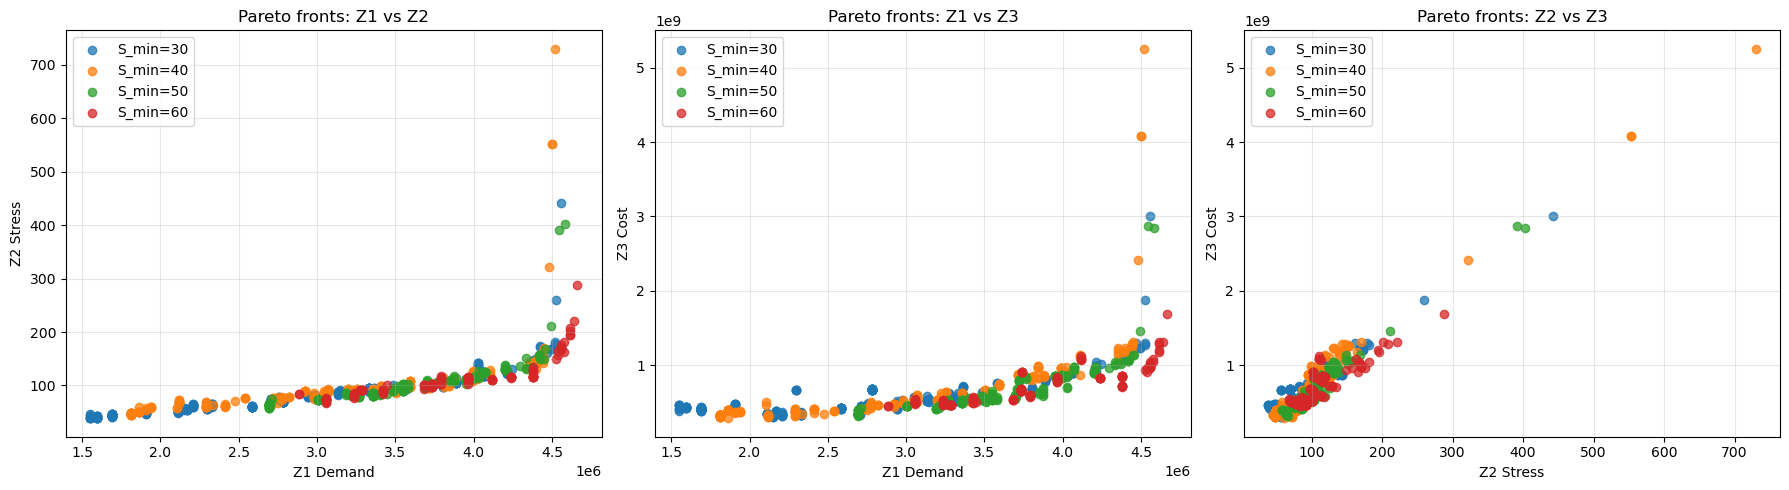
\includegraphics[width=\textwidth]{Figures/Sensitivity_Plots_2D_Pop_1200_V3.png}
  \caption{Pairwise projections of the NSGA-II Pareto set showing sensitivity to the minimum number of stations.}
  \label{fig:Sen_pareto_2d}
\end{figure}

\begin{table}[htbp]
  \caption{Sensitivity analysis results for different minimum link constraints ($M_{\min}$).}
  \label{tab:sensitivity_mmin}
  \centering
  \small
  \begin{tabular}{@{}lcccc@{}}
    \hline
    \textbf{$M_{\min}$} & \textbf{50} & \textbf{100} & \textbf{150} & \textbf{200} \\
    \hline
    Max Z1 (million) & 4.953 & 4.851 & 4.711 & 4.820 \\
    Min Z2 & 87.19 & 158.39 & 247.92 & 330.80 \\
    Min Z3 (million) & 5.24 & 8.65 & 12.95 & 16.37 \\
    \hline
  \end{tabular}
\end{table}

\begin{figure}[htbp]
  \centering
  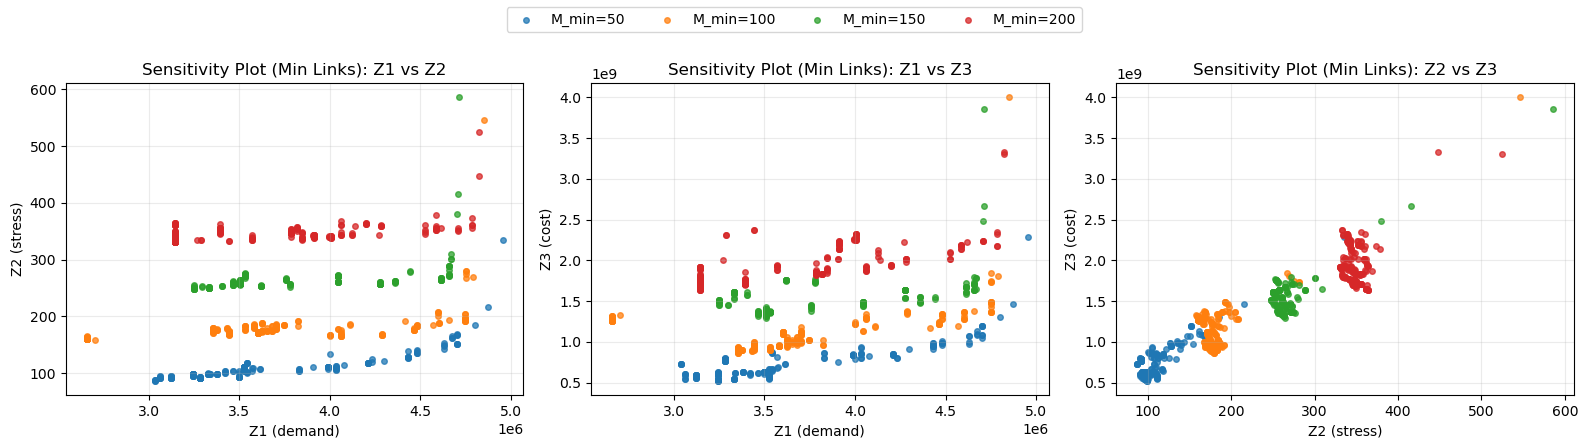
\includegraphics[width=\textwidth]{Figures/Sensitivity_Links_Plots_2D_Pop_1200.png}
  \caption{Pairwise projections of the NSGA-II Pareto set showing sensitivity to the minimum number of links.}
  \label{fig:Sen_pareto_2d_links}
\end{figure}

% References are now handled by the elsarticle class
% The bibstyle is changed to elsarticle-num
\bibliographystyle{elsarticle-harv}
\bibliography{trb_template}
% References
\end{document}
